%%%  Založeno na stylu pro text závěrečné (bakalářské a
%%%  diplomové) práce na KI PřF UP v Olomouci
%%%  Copyright (C) 2012 Martin Rotter, <rotter.martinos@gmail.com>
%%%  Copyright (C) 2014 Jan Outrata, <jan.outrata@upol.cz>

\documentclass[
  biblatex,
%  figures=false,
  sourcecodes,
  glossaries,
  index
]{kidiplom}

\usepackage{graphicx}
\usepackage{float}
\graphicspath{ {./graphics/} }

%% Název práce, česky a anglicky
\title{Nástroj pro analýzu DBLP databáze}
\title[english]{DBLP database analysis tool}

%% Jméno autora práce
\author{Radek Vymětalík}

%% Jméno vedoucího práce (včetně titulů)
\supervisor{RNDr. Martin Trnečka, Ph.D.}

%% Volitelný rok odevzdání práce. Výchozí je aktuální (kalendářní)
%% rok
%\yearofsubmit{\the\year}

%% Anotace práce, včetně anglické (obvykle překlad z jazyka
%% práce). Jeden odstavec!
\annotation{Bakalářská práce se zabývá vývojem webové aplikace pro analýzu DBLP databáze -- přední databáze metadat publikací z~různých oblastí informatiky. Práce nejprve seznamuje čtenáře s~obsahem DBLP databáze a~možnostmi jeho stažení. Následně popisuje použité technologie, motivaci pro jejich zvolení a~implementační aspekty aplikace včetně její architektury a~klíčových komponent. Ke konci práce je uveden postup zprovoznění aplikace a~její uživatelská příručka.}

\annotation[english]{The~bachelor’s thesis deals with the development of a~web application for analyzing the DBLP database -- a~leading database of publication metadata from various fields of computer science. The~thesis first introduces readers to the content of the DBLP database and its download options. Subsequently, it describes the technologies used, the motivation for their selection, and the implementation aspects of the~application, including its architecture and key components. The~end of the thesis provides instructions for setting up the application and its user guide.}

%% Klíčová slova práce, včetně anglických. Oddělená (obvykle) středníkem.
\keywords{webová aplikace; DBLP; vizualizace dat; Next.js}
\keywords[english]{web application; DBLP; data visualization; Next.js}

%% Volitelná specifikace příloh textu práce, i anglicky. Výchozí je
%% 'elektronická data v systému katedry informatiky / electronic data
%% in system of department of computer science'.
%\supplements{nejlepší software všech dob}
%\supplements[english]{the best software of all times}

%% Volitelné poděkování. Stručné! Výchozí je prázdné. Makro nemá
%% nepovinný parametr pro uvedení jazyka.
\thanks{Děkuji vedoucímu bakalářské práce RNDr. Martinu Trnečkovi, Ph.D. za jeho odborné vedení, čas a poskytnuté rady.}

%% Cesta k souboru s bibliografií pro její sazbu pomocí BibLaTeXu
%% (zvolenou nepovinným parametrem biblatex makra
%% \documentclass). Použijte pouze při této sazbě, ne při (výchozí)
%% sazbě v prostředí thebibliography.
\bibliography{bibliografie.bib}

%% Další dodatečné styly (balíky) potřebné pro sazbu vlastního textu
%% práce.
\usepackage{lipsum}
\usepackage{longtable}

\begin{document}
%% Sazba úvodních stran -- titulní, s bibliografickými údaji, s
%% anotací a klíčovými slovy, s poděkováním a prohlášením, s obsahem a
%% se seznamy obrázků, tabulek, vět a zdrojových kódů (pokud jejich
%% sazba není vypnutá).
\maketitle

%% Vlastní text závěrečné práce. Pro povinné závěry, před přílohami,
%% použijte prostředí kiconclusions. Povinná je i příloha s obsahem
%% elektronických dat.

%% -------------------------------------------------------------------

\newcommand{\BibLaTeX}{\textsc{Bib}\LaTeX}

\section{Úvod}

DBLP Computer Science Bibliography, nebo jen DBLP, je přední veřejně přístupná databáze a~webová služba poskytující metadata publikací z~různých oblastí informatiky. Nalezneme v~ní nejen publikace z~mnoha významných časopisů a~sborníků konferencí, ale~i~vědecké monografie a~encyklopedie. V~roce 2024 databáze obsahuje více než 7~milionů publikací od více než 3~milionů autorů z~celého světa~\cite{t00}. Nová data jsou do databáze neustále přidávána poloautomatickým procesem pod dohledem výzkumného centra Schloss Dagstuhl, které se snaží zaručit co nejvyšší kvalitu těchto dat.

DBLP poskytuje hodnotná data pro mnohé výzkumné pracovníky a~instituce. Pro snadnější pochopení, srovnávání, sledování trendů a~celkovou analýzu by však bylo vhodné mít možnost tato data a~vztahy mezi nimi přehledně prezentovat. Právě k~takovým účelům slouží online nástroj vytvořený v~rámci této bakalářské práce. Pomocí různých typů grafů a~tabulek přehledně prezentuje data stažená z~databáze, především tedy metadata autorů, časopisů a~konferencí. Nástroj umožňuje:
\begin{itemize}
\item vizualizovat statistiky autorů, časopisů nebo konferencí pomocí různých typů grafů,
\item prohlížet metadata publikací s~možností jejich filtrování,
\item vytvářet skupiny autorů, prezentovat jejich statistiky a~provádět nad nimi jednoduchou analýzu,
\item vizualizovat grafy spoluautorství s~možností filtrování zobrazených autorů podle různých parametrů,
\item exportovat analyzovaná data.
\end{itemize}

\newpage

\section{Obsah DBLP}

Všechen obsah DBLP databáze je přístupný skrze webovou službu, kterou nalezneme na adrese \href{https://dblp.org/}{https://dblp.org/}. Na této adrese jsou k~dispozici jak webové stránky umožňující databázi pohodlně prohledávat, tak i~volně dostupné webové API. Všechna data v~databázi jsou zveřejněna pod licencí CC0 1.0 Public Domain Dedication license. Tato data tedy můžeme volně distribuovat, kopírovat, upravovat, přetvářet a vytvářet z~nich odvozená díla, a~to i~pro komerční účely a~bez vyžádání svolení~\cite{t01}.

\subsection{Základní typy stránek}

Základní strukturu webové stránky tvoří pět typů stránek:
\begin{itemize}
\item stránky abecedně uspořádaných indexů,
\item stránky proudů publikací,
\item stránky svazků (obsahů),
\item stránky jednotlivých publikací,
\item stránky jednotlivých autorů.
\end{itemize}

Indexů nabízí webová stránka hned několik. Nejvýznamnějšími jsou index vědeckých časopisů, index konferencí a~workshopů a~index sérií. Série sdružují tématicky související publikace, třeba i~z~různých časopisů nebo konferencí. V~těchto indexech jsou uvedeny odkazy na stránky \textit{proudů publikací}, taktéž označovaných jako venues. Těmi se rozumí konkrétní vědecké časopisy, konference, workshopy nebo~série. Na stránkách proudů publikací pak nalezneme odkazy na stránky \textit{svazků}, které představují například jednotlivé svazky časopisů a~konferencí nebo obsahy monografií.

Na~stránkách svazků jsou uvedena metadata publikací. V~mnoha případech jsou však metadata publikací uvedena již na~stránce proudu publikací. Takové publikace většinou samy reprezentují stránky svazků a~slouží jako odkazy na~ně. Taktéž se může jednat o~proudy publikací, které se již dále nedělí na~svazky. Odkazy mezi zmíněnými stránkami a~metadaty publikací můžeme vidět znázorněny na~obrázku~\ref{fig:typy_stranek_odkazy}.

\begin{figure}[H]
\begin{center}
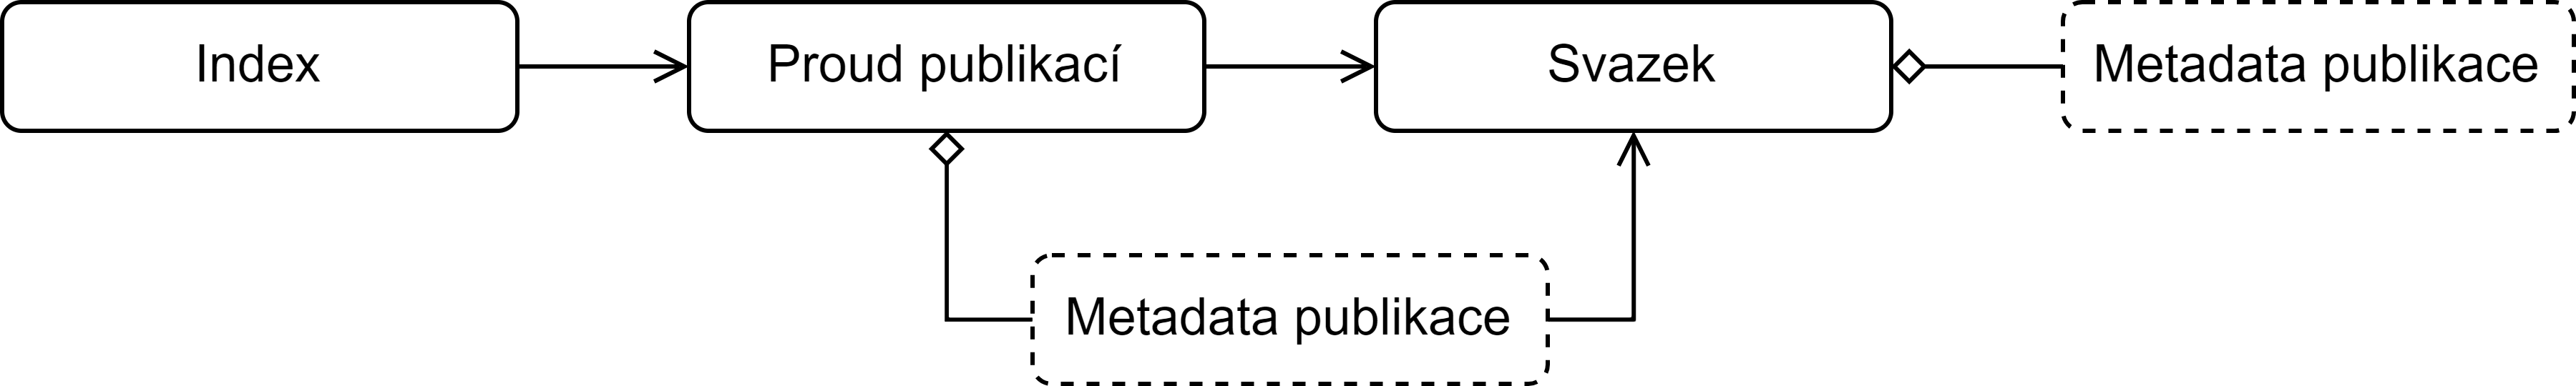
\includegraphics[width=\textwidth]{typy_stranek_odkazy}
\caption{Odkazy mezi stránkami a~metadaty publikací v~DBLP}\label{fig:typy_stranek_odkazy}
\end{center}
\end{figure}

Všechna metadata publikace taktéž najdeme na samostatné stránce dané publikace. Na této stránce si lze navíc nechat načíst dodatečná metadata, která nejsou uložena v databázi, ze~služeb OpenAlex~\cite{t02}, Crossref~\cite{t03}, OpenCitations~\cite{t04} a~Semantic~Scholar~\cite{t05}. Těmito metadaty jsou především:
\begin{itemize}
\item reference publikace,
\item citace publikace,
\item obsažené pojmy.
\end{itemize}

Všichni autoři uložení v~databázi jsou dohledatelní skrze index autorů obsahující odkazy na stránky jednotlivých autorů. Na~stránce autora jsou uvedeny jeho základní informace, jako například jméno, příslušnost k~univerzitě nebo dosažená ocenění, a~metadata všech jeho publikací nacházejících se v~databázi. Na~obrázku~\ref{fig:michael_ley_dblp} můžeme vidět část stránky autora Michael Ley~\cite{t07}.

\begin{figure}[H]
\begin{center}
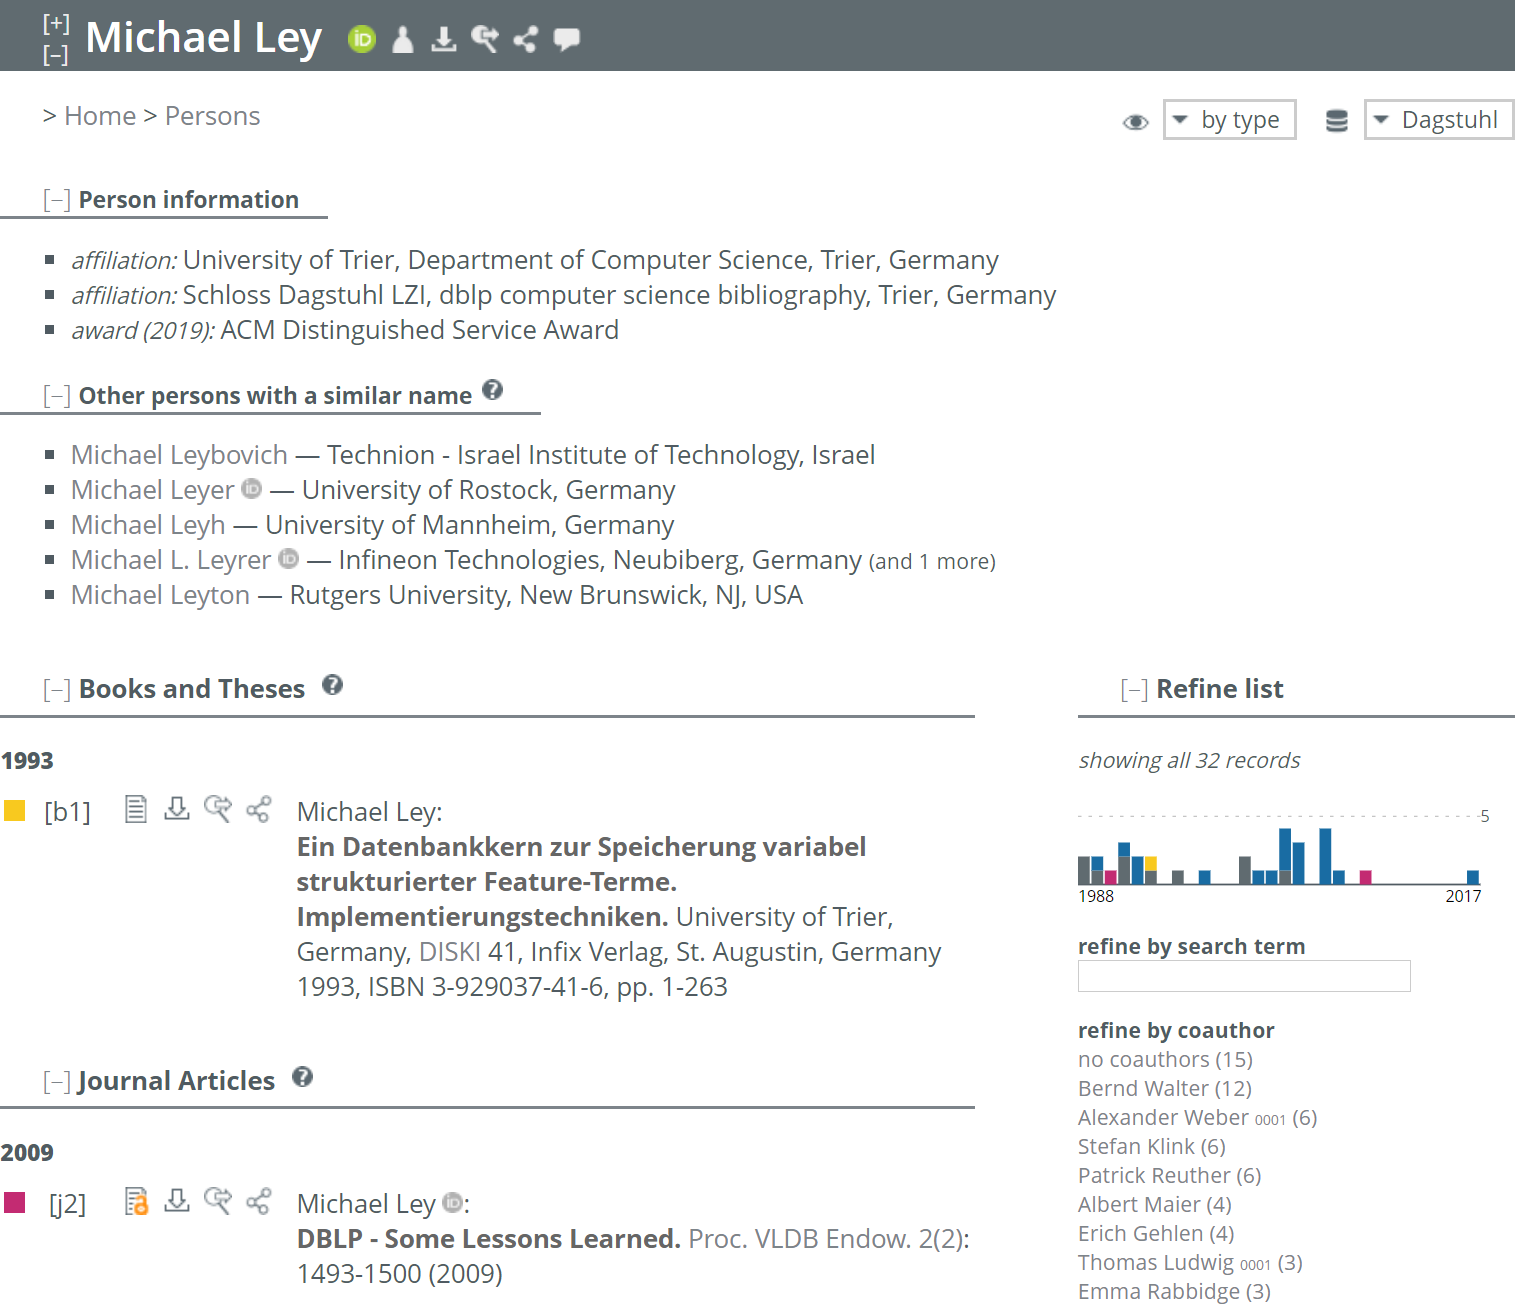
\includegraphics[width=\textwidth]{michael_ley_dblp}
\caption{Část stránky autora Michael Ley v~DBLP}\label{fig:michael_ley_dblp}
\end{center}
\end{figure}

\subsection{URL adresy základních typů stránek}

Na obrázku~\ref{fig:struktura_url_adres_dblp} můžeme vidět znázorněnu organizaci všech doposud zmíněných typů stránek z~pohledu jejich URL adres. Kromě stránek indexů je obsah všech uvedených stránek k dispozici jak ve formátu HTML, tak i~ve formátu XML. Identifikátor publikace, nebo též klíč, se skládá z~několika segmentů. Úvodní segmenty typicky označují proud publikací, do kterého je publikace zařazena. Neplatí~to však pro všechny publikace. Obdobně se i~identifikátory autorů skládají z~více segmentů.

\begin{figure}[H]
\begin{center}
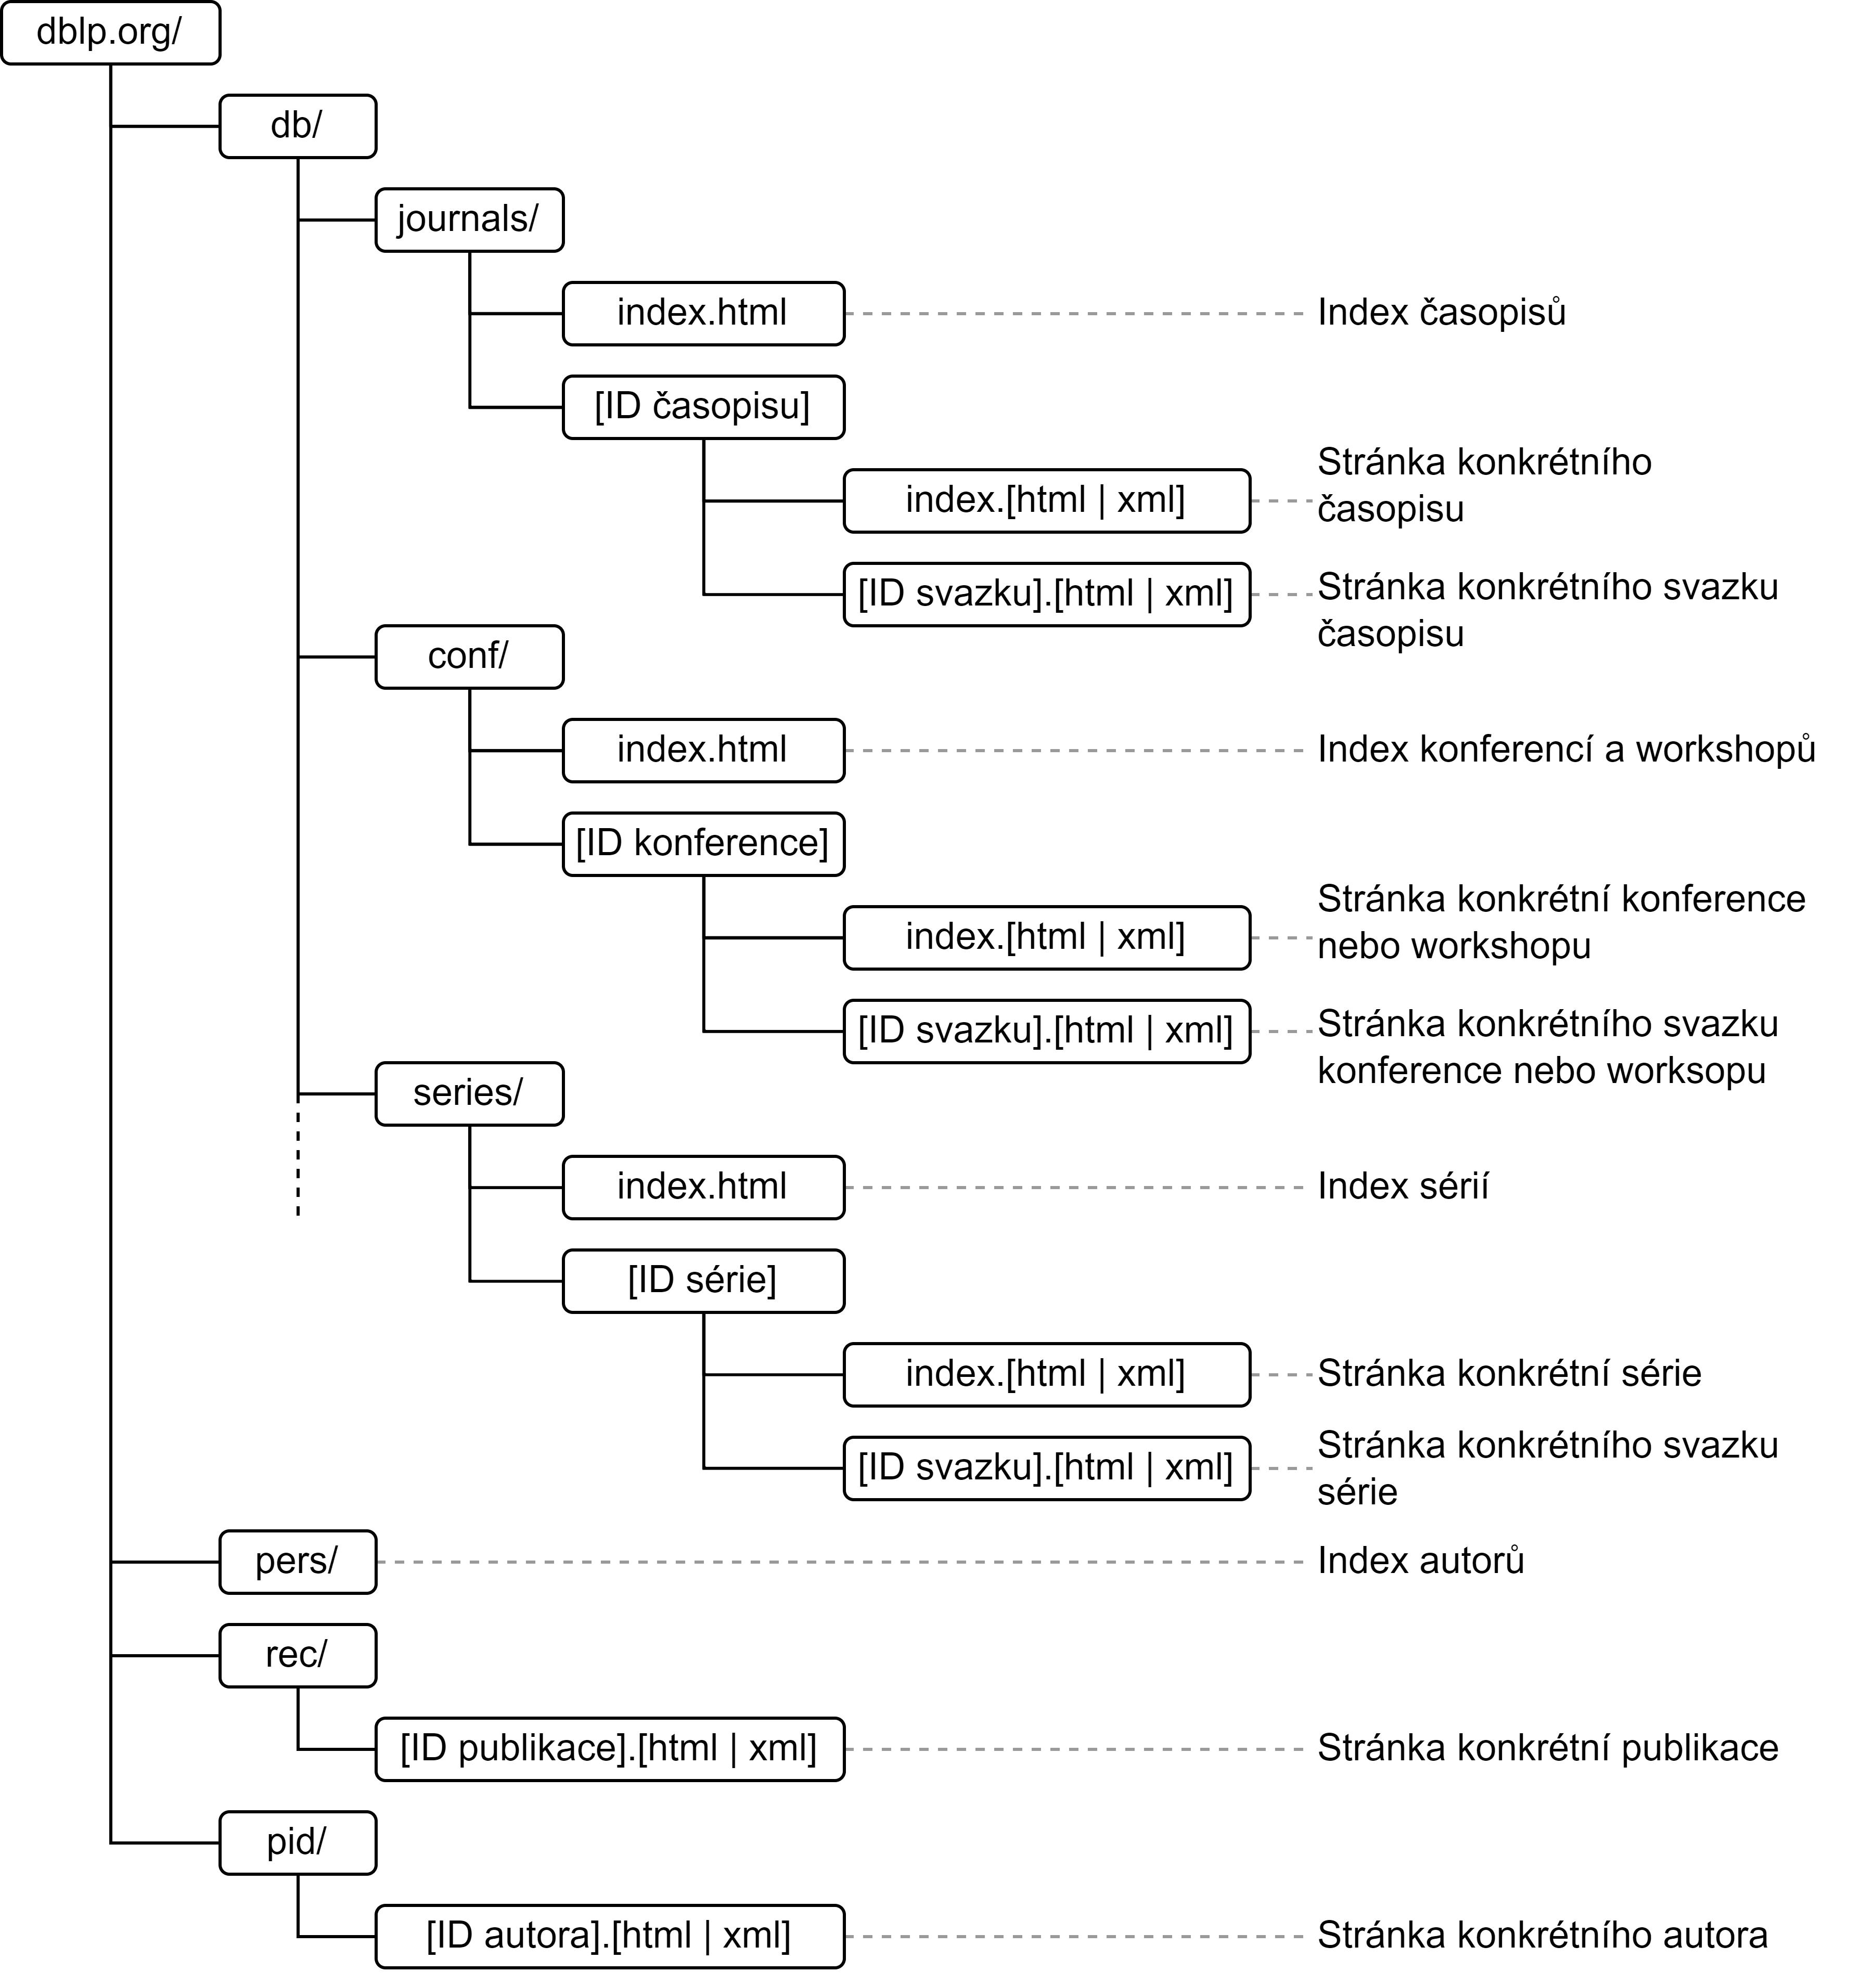
\includegraphics[width=\textwidth]{dblp_urls}
\caption{Struktura webové stránky DBLP}\label{fig:struktura_url_adres_dblp}
\end{center}
\end{figure}

\subsection{Vyhledávání}

Pro snadnější prohledávání obsahu databáze poskytuje DBLP na svých webových stránkách vlastní vyhledávač založený na řešení jménem CompleteSearch~\cite{t08}. Výsledkem vyhledávání je buď:
\begin{itemize}
\item seznam s odkazy na stránky autorů,
\item seznam s odkazy na stránky proudů publikací,
\item nebo seznam metadat publikací.
\end{itemize}

Ve výchozím nastavení vyhledávání zobrazí stránku s~kombinací všech těchto typů výsledků. Je~však možné si nechat zobrazit jen jeden určitý typ výsledku. Výsledek vyhledávání vždy obsahuje nejvýše prvních~1000 vyhovujících záznamů. Na~obrázku~\ref{fig:struktura_url_adres_vyhledavani_dblp} můžeme vidět organizaci stránek s~výsledky vyhledávání z~pohledu jejich URL adres.

\begin{figure}[H]
\begin{center}
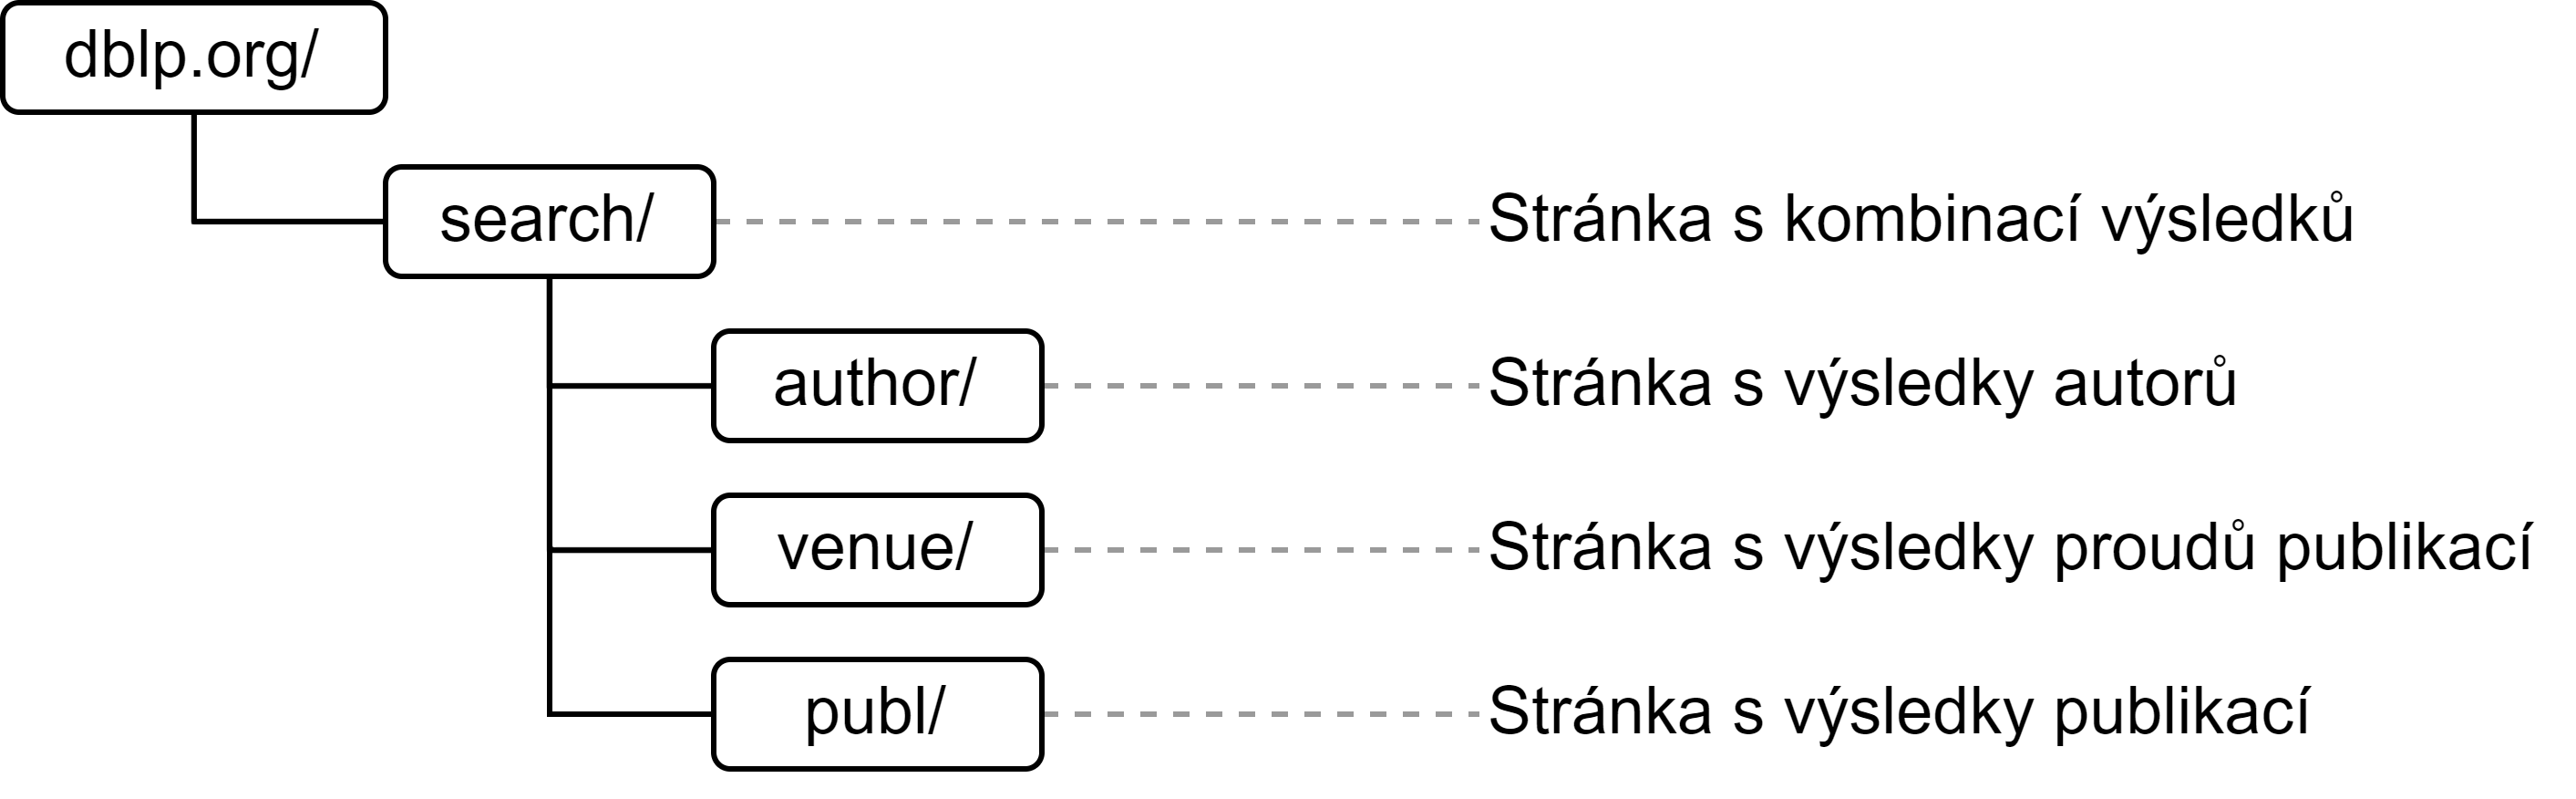
\includegraphics[width=12cm]{vyhledavani_dblp_urls}
\caption{Stránky s~výsledky vyhledávání v~DBLP}\label{fig:struktura_url_adres_vyhledavani_dblp}
\end{center}
\end{figure}

Ve výchozím nastavení vyhledávač porovnává každý hledaný výraz jako předponu potenciálního výsledku vyhledávání. Jestliže hledaný výraz obsahuje více slov oddělených prázdným znakem (například mezera nebo tabulátor) nebo znakem \uv{+}, pak všechny musí být předponami v~hledaném výsledku. Nerozlišují se velká a~malá písmena a~ani~diakritika. Vyhledávání není fulltextové. Porovnávají se pouze některá metadata uložená v~databázi, především tedy názvy publikací, proudů publikací a~jména autorů. Možnosti konstrukce hledaných výrazů můžeme vidět v~tabulce~\ref{tab:moznosti_konstrukce_hledanych_vyrazu}, kterou jsem převzal z~FAQ sekce DBLP~\cite{t09}.

\begin{table}[h]
\begin{center}
\caption{Možnosti konstrukce hledaných výrazů v~DBLP}\label{tab:moznosti_konstrukce_hledanych_vyrazu}
\begin{tabular}{|L{4cm}|L{4cm}|L{5cm}|}
\hline
\textbf{Možnost} & \textbf{Syntax} & \textbf{Příklad} \\
\hline
prefixové hledání & výchozí & \uv{sig} se shoduje se slovem \uv{SIGIR} a~také \uv{signal} \\
\hline
přesné hledání & znak \uv{\$} za hledaným výrazem & \uv{graph\$} se shoduje se slovem \uv{graph}, ale~ne~s~\uv{graphics} \\
\hline
booleovské AND & slova oddělená prázdným znakem nebo znakem \uv{+} & \uv{codd model} se shoduje jak s~výrazem \uv{Codd's Relational Model}, tak i~\uv{A Model by Codd} \\
\hline
booleovské OR & slova oddělená znakem \uv{|} & \uv{graph|network} se shoduje jak s~\uv{graph algorithm}, tak i~\uv{Network Analysis} \\
\hline
\end{tabular}
\end{center}
\end{table}

%% https://dblp.org/faq/16154928.html - není fulltextové

\subsection{Vyhledávání pomocí API}

Stejné řešení vyhledávání, které lze použít na webových stránkách DBLP, je přístupné i~skrze veřejné API. Toto API poskytuje tři koncové body pro vyhledávání autorů, publikací a~proudů publikací. URL adresy těchto koncových bodů jsou znázorněny na~obrázku~\ref{fig:struktura_url_adres_vyhledavani_dblp_api}. Výsledek vyhledávání můžeme ovlivnit několika parametry, jejichž výchozí hodnoty a příklady nalezneme v~tabulce~\ref{tab:parametry_vyhledavani_api_dblp}.

Hledaný výraz definujeme parametrem \texttt{q} URL adresy. Při~konstrukci hledaného výrazu můžeme využít všechny možnosti uvedené v~tabulce~\ref{tab:moznosti_konstrukce_hledanych_vyrazu}.

Parametrem \texttt{h} můžeme nastavit maximální povolený počet vrácených záznamů. V~kombinaci s~parametrem \texttt{f}, kterým definujeme hodnotu pořadí prvního vráceného prvku (pořadí je počítáno od nuly), je možné implementovat stránkování záznamů. Omezením tohoto API však je, že umožňuje vrátit najednou nejvýše 1000 záznamů, a to pouze z~prvních nejvýše 10000 nalezených záznamů. K~více než prvním 10000 vyhovujících záznamů se tedy nedostaneme.

\begin{figure}[H]
\begin{center}
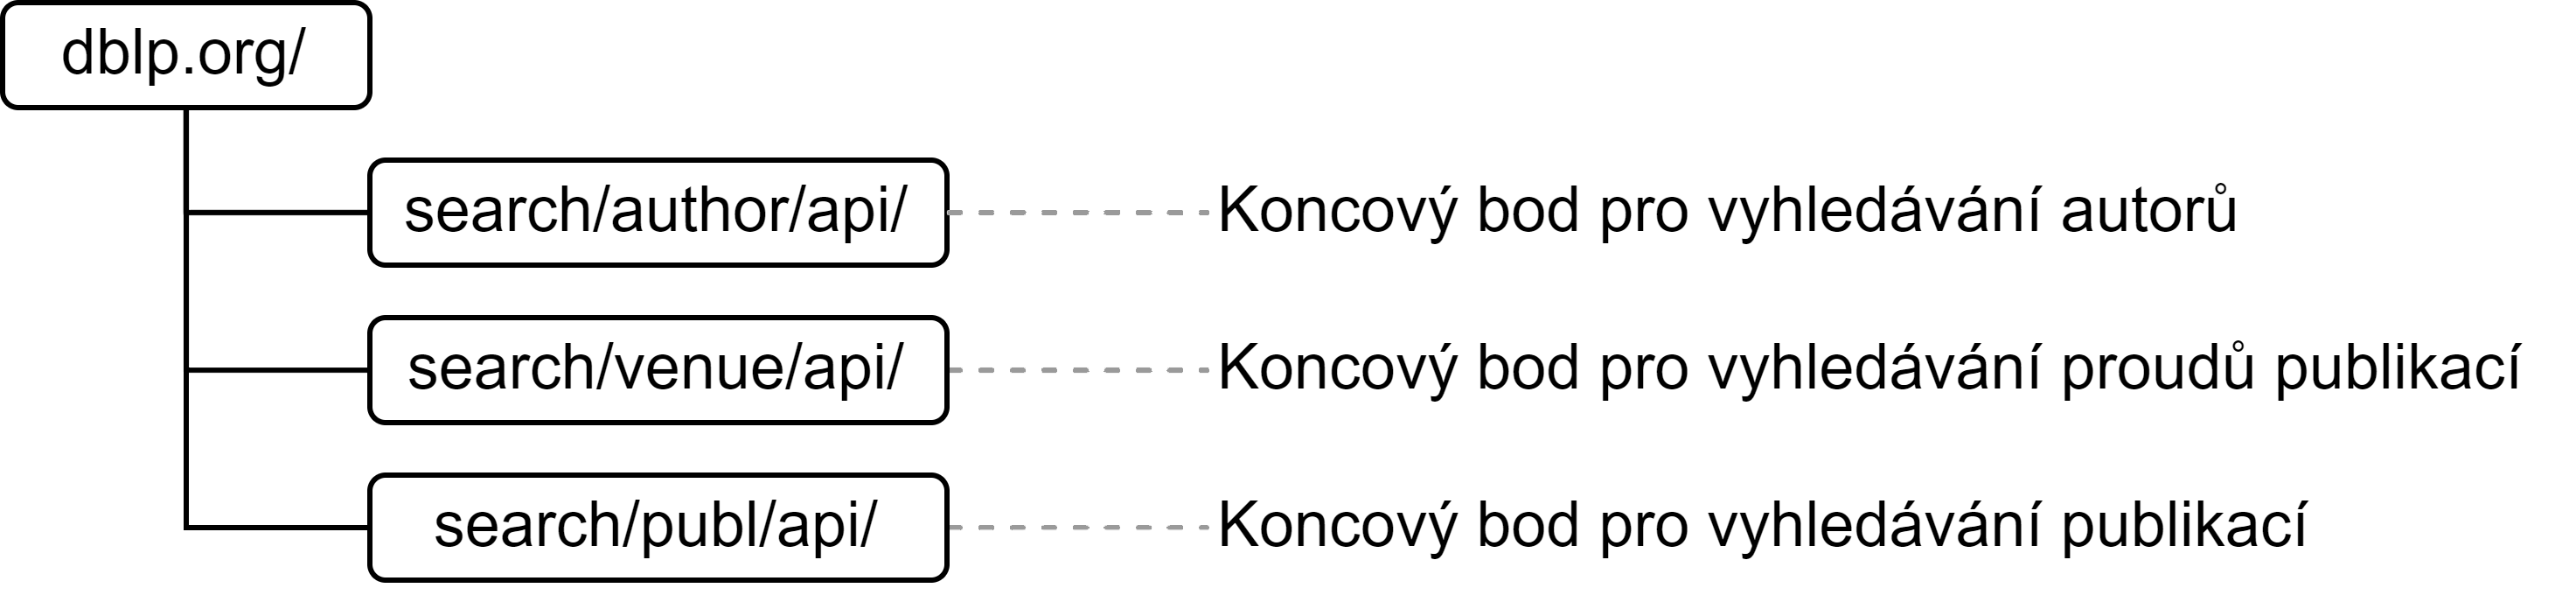
\includegraphics[width=12.5cm]{vyhledavani_dblp_api_urls}
\caption{URL adresy koncových bodů pro vyhledávání v~DBLP}\label{fig:struktura_url_adres_vyhledavani_dblp_api}
\end{center}
\end{figure}

API vrací vedle konkrétních záznamů shodujících se s~hledaným výrazem ještě i~seznam celých slov, jejichž prefixem je slovo uvedené nejvíce napravo v~hledaném výrazu. Jde tedy o~slova, na která lze hledaný výraz doplnit. Maximální povolený počet takových slov, která API může vrátit, nastavíme parametrem~\texttt{c}.

Formát vrácených dat definujeme parametrem \texttt{format}, který přijímá hodnoty:
\begin{itemize}
\item \texttt{xml} pro formát XML,
\item \texttt{json} pro formát JSON,
\item \texttt{jsonp} pro formát JSONP.
\end{itemize}

\begin{table}[h]
\begin{center}
\caption{Parametry URL adres koncových bodů API pro vyhledávání v~DBLP}\label{tab:parametry_vyhledavani_api_dblp}
\begin{tabular}{|L{2cm}|L{2cm}|L{9cm}|}
\hline
\textbf{Parametr} & \textbf{Výchozí hodnota} & \textbf{Příklad} \\
\hline
\texttt{q} &  & \href{https://dblp.org/search/author/api?q=jan+novak}{\texttt{.../author/api?q=jan+novak}} \\
\hline
\texttt{h} & \texttt{30} & \href{https://dblp.org/search/author/api?q=jan&h=200}{\texttt{.../author/api?q=jan\&h=200}} \\
\hline
\texttt{f} & \texttt{0} & \href{https://dblp.org/search/author/api?q=jan&h=200&f=9000}{\texttt{.../author/api?q=jan\&h=200\&f=9000}} \\
\hline
\texttt{c} & \texttt{10} & \href{https://dblp.org/search/author/api?q=jan&c=30}{\texttt{.../author/api?q=jan\&c=30}} \\
\hline
\texttt{format} & \texttt{xml} & \href{https://dblp.org/search/author/api?q=jan&format=json}{\texttt{.../author/api?q=jan\&format=json}} \\
\hline
\end{tabular}
\end{center}
\end{table}

\subsection{Metadata publikací}

Celý dataset s~metadaty publikací je k~dispozici ke stažení jako XML soubor \texttt{dblp.xml}, který je umístěný v adresáři na adrese \href{https://dblp.org/xml/}{https://dblp.org/xml/}. Formát tohoto souboru je definován v~DTD souboru \texttt{dblp.dtd}, který se nachází ve stejném adresáři. Stejný formát pro reprezentaci metadat publikací je použit i~v~XML souborech stránek proudů publikací, svazků, publikací a autorů. Detailnější informace o souboru \texttt{dblp.xml} a~jeho formátu nalezneme ve~FAQ~sekci~DBLP~\cite{t10}.

Metadata všech publikací vždy obsahují:
\begin{itemize}
\item unikátní identifikátor,
\item název,
\item typ publikace.
\end{itemize}

Volitelně (typicky v~závislosti na typu publikace) pak metadata obsahují ještě například:
\begin{itemize}
\item seznam autorů nebo editorů,
\item rok zveřejnění,
\item název a~identifikátor proudu publikací,
\item název vydavatele,
\item jeden nebo více odkazů na~digitální vydání publikace,
\item počet stránek.
\end{itemize}

DBLP uchovává metadata publikací několika typů. Typy publikací, které jsou prezentované uživateli a~jejichž přehled můžeme vidět v~tabulce~\ref{tab:typy_publikaci}, však nejsou úplně totožné s~typy, pod kterými jsou metadata uložená v~souboru \texttt{dblp.xml}. Metadata publikací jednotlivých typů, která se nachází v~souboru \texttt{dblp.xml}, jsou inspirována typy záznamů formátu BibTeX. Konkrétně se jedná o~následující typy záznamů:
\begin{itemize}
\item \texttt{article} -- článek recenzovaného časopisu,
\item \texttt{inproceedings} -- příspěvek recenzované konference nebo workshopu,
\item \texttt{proceedings} -- svazek recenzované konference nebo workshopu,
\item \texttt{book} -- monografie,
\item \texttt{incollection} -- kapitola monografie,
\item \texttt{phdthesis} -- doktorská práce,
\item \texttt{mastersthesis} -- diplomová práce,
\item \texttt{www} -- webová stránka.
\end{itemize}

%% Doplnit reference z tudma? https://bibtex.eu/types/

Kromě těchto typů autoři DBLP ještě zavedli vlastní typ~\texttt{data}~\cite{t11}. Tento typ je určen pro datasety a~artefakty.

%% https://dblp.org/faq/16154937.html

%% https://dblp.org/xml/docu/dblpxml.pdf

\begin{table}[h]
\begin{center}
\caption{Typy publikací v~DBLP}\label{tab:typy_publikaci}
\begin{tabular}{|L{4cm}|L{9cm}|}
\hline
\textbf{Anglické označení} & \textbf{Český popis} \\
\hline
Books and Theses & monografie a~vysokoškolské práce \\
\hline
Journal Articles & články, úvodní slova a~předmluvy recenzovaných časopisů \\
\hline
Conference and Workshop Papers & příspěvky recenzovaných konferencí nebo workshopů \\
\hline
Parts in Books or Collections & výzkumné články, které byly vydány jako kapitola monografie \\
\hline
Editorship & editované publikace a sborníky \\
\hline
Reference Works & referenční materiály, výzkumné práce a~encyklopedie \\
\hline
Data and Artifacts & datasety a~artefakty (jako například software) \\
\hline
Informal and Other Publications & neformální a~zbylé publikace typicky zveřejněné v~online repositářích bez přísného prověřovacího procesu nebo na neformálních workshopech \\
\hline
\end{tabular}
\end{center}
\end{table}

%% https://dblp.org/faq/1474794.html

\subsection{Možnosti stažení dat} \label{sec:moznosti_stazeni_dat}

Z~předchozích řádků plyne, že DBLP poskytuje několik možností, jak můžeme data z~databáze stáhnout pro vlastní potřeby. Každá má své výhody i~nevýhody:

\begin{itemize}
\item Stažení datasetu publikací -- Jednou z~možností je si stáhnout celý dataset publikací najednou jako jeden XML soubor. Zde je výhodou vysoká flexibilita. Nijak nás neomezuje podoba a~vlastnosti API, které DBLP poskytuje, a~můžeme s~daty pracovat jakkoliv potřebujeme. Nevýhodou však je, že dataset obsahuje pouze metadata publikací. Například podrobnější informace o~autorech, jako je identifikátor, dosažená ocenění nebo příslušnost k~univerzitě, v~něm nenajdeme. Dále si dataset musíme sami pravidelně obnovovat, abychom vždy pracovali s~aktuálními daty. Taktéž si musíme sami implementovat všechny operace nad daty, jako například vyhledávání nebo seskupování publikací do proudů publikací.
\item Stažení stránek ve formátu HTML -- Při použití tohoto přístupu se dostaneme ke všem datům, ke kterým se dostane běžný uživatel webové stránky. Data stahujeme ve formě HTML souborů. Ty ale často obsahují i~množství nerelevantních informací, což může komplikovat extrahování námi požadovaných dat.
\item Stažení stránek ve formátu XML -- Další možností je stránky stahovat ve formátu XML, který neobsahuje tolik nepodstatných informací. Zde je největší nevýhodou, že DBLP podporuje tuto možnost pouze pro některé typy stránek, konkrétně tedy jen pro stránky proudů publikací, svazků, publikací a~autorů.
\item Využití API pro vyhledávání -- Toto řešení je ideální pro implementaci vyhledávání v databázi. Zásadním omezením však může být nemožnost získat více jak prvních 10000 vyhovujících záznamů.
\end{itemize}

Dalším omezením, na které je potřeba si dávat pozor především u~posledních tří zmíněných možností, je omezení na počet požadavků, které lze za určitý časový interval poslat. V~případě vysokého vytížení služby může DBLP vracet prázdnou odpověď se stavovým HTTP kódem 429. Z~tohoto důvodu autoři DBLP doporučují čekat mezi dvěma po sobě následujícími požadavky alespoň jednu nebo dvě sekundy~\cite{t12}.

%% https://developer.mozilla.org/en-US/docs/Web/HTTP/Status/429

\newpage

\section{Použité technologie}

Nástroj pro analýzu DBLP databáze jsem implementoval jako webovou aplikaci pomocí frameworku Next.js verze~14~\cite{t13} a~řady dalších technologií. Jedním~z~hlavních faktorů, podle kterých jsem se při volbě použitých technologií rozhodoval, byla jejich popularita. Tu~jsem alespoň orientačně určoval podle počtu stažení odpovídajících balíčků. Celou aplikaci jsem napsal v~editoru Visual Studio Code a~testoval ji ve webových prohlížečích:
\begin{itemize}
\item Google Chrome,
\item Firefox,
\item Safari.
\end{itemize}

\subsection{Framework Next.js}

Next.js je framework postavený na knihovně React~\cite{t14}, který zjednodušuje vývoj webových aplikací. Umožňuje pomocí jedné technologie vyvíjet jak serverovou, tak i~klientskou část aplikace. Základem jsou React komponenty, které slouží ke tvorbě uživatelského rozhraní. Next.js tyto komponenty doplňuje o~další funkcionality a~optimalizace. Pro vykonávání kódu na straně serveru používá Next.js běhové prostředí Node.js. Funkcionality a~vlastnosti, kvůli kterým jsem se rozhodl pro tento framework, jsou:
\begin{itemize}
\item Sever-side rendering -- React komponenty je možné renderovat zcela, nebo jen částečně na straně serveru, a~to buď staticky při sestavování aplikace, anebo dynamicky za běhu. Díky tomuto přístupu uživatel vždy vidí aspoň část obsahu stránky ještě před tím, než se vykoná jakýkoliv JavaScript kód v prohlížeči, což vede ke příjemnějšímu uživatelskému zážitku.
\item App Router -- Systém řešící mapování URL adres na jednotlivé stránky aplikace. Toto mapování je určené pouze adresářovou strukturou, kde každý adresář reprezentuje jeden segment cesty URL adresy.
\item Rozšířené \texttt{fetch} API -- Next.js automaticky ukládá do mezipaměti (cache) odpovědi na požadavky, které jsou posílány pomocí \texttt{fetch} API na straně serveru. V případě opakovaného zasílání požadavku na stejnou adresu vrací data uložená v mezipaměti. Tím se snižuje množství zasílaných požadavků na další služby.
\item TypeScript -- Next.js má vestavěnou podporu jazyka TypeScript~\cite{t15}, který je rozšířením jazyka JavaScript o~statickou kontrolu datových typů. Statická kontrola datových typů mi umožnila odhalit množství chyb ještě při psaní kódu a~minimalizovat tak problémy za běhu aplikace. Zároveň považuji za výhodu, že jsem celou aplikaci mohl napsat v~jednom jediném programovacím jazyce.
\item Modularita -- Koncept React komponent umožňuje rozdělit aplikaci na menší, nezávislé a znovupoužitelné části s~jasně definovaným účelem. Komponenty lze definovat buď jako funkce, nebo jako třídy. Já jsem zvolil definici pomocí funkcí, protože mi připadne jednodušší a~přehlednější. Pro sdílení funkcionality mezi komponentami jsou v~tomto případě k~dispozici tzv.~React~hooks. Opět jde o~funkce, které pouze zapouzdřují požadovanou logiku a~které voláme v~komponentách. React poskytuje sadu základních React~hooks (například \texttt{useState()} pro uchování stavu komponenty). Můžeme si však definovat i~vlastní nebo využít balíčků třetích stran s~již předdefinovanými React hooks. Já~se~rozhodl použít balíček usehooks-ts~\cite{t16}, který poskytuje mnoho React hooks pro jednodušší práci například s~událostmi nebo úložištěm prohlížeče.
\end{itemize}

Pokud funkce nepracuje s~API specifickým pouze pro prohlížeč nebo naopak s~API specifickým pouze pro Node.js, tak ji můžeme volat na straně klienta i~na straně serveru. Když potřebuji, aby taková funkce mohla být zavolána pouze na straně serveru, tak používám balíček server-only~\cite{t17}. Balíček zajistí, že obsah souboru, do kterého je tento balíček naimportovaný, můžeme použít pouze na straně serveru.

\subsection{Databázový systém MongoDB}

Na straně serveru jsem se rozhodl implementovat vlastní řešení mezipaměti postavené na databázovém systému MongoDB~\cite{t18}. Do této paměti ukládám stažené záznamy z~DBLP. Mezipaměť poskytovaná frameworkem Next.js totiž umožňuje uložení pouze záznamů, jejichž velikost nepřesahuje~2~MB.

MongoDB je NoSQL databázový systém, který ukládá data ve formě dokumentů formátu BSON (formát podobný JSON). Umožňuje mít flexibilní schémata, která je možné jednoduše měnit a~integrovat s~aplikacemi.

Pro přístup k~MongoDB z~aplikace jsem zvolil knihovnu Mongoose~\cite{t19} určenou pro použití s~Node.js. V~jazyce JavaScript, respektive TypeScript, lze díky této knihovně na databázi nejen volat dotazy pro manipulaci s~daty, ale~i~definovat databázová schémata. Integrovat MongoDB do Next.js aplikace tak pro mě bylo velmi snadné.

\subsection{Knihovna SWR}

Pro načítání dat ze serveru nebo přímo z~DBLP na straně klienta jsem se rozhodl použít knihovnu SWR~\cite{t20}. SWR poskytuje sadu předpřipravených React hooks, které mimo jiné řeší automatické ukládání dat do mezipaměti a~zpracování stavů HTTP požadavků. Výrazně tak zjednodušuje logiku načítání dat a~díky mezipaměti snižuje množství posílaných požadavků.

\subsection{Knihovna Cheerio}

Extrahování dat z dokumentů ve formátu HTML nebo XML na straně serveru řeším pomocí knihovny Cheerio~\cite{t21}. Tato knihovna převádí HTML nebo XML dokumenty na jednoduchý objektový model (DOM) a~poskytuje rozhraní silně inspirované knihovnou jQuery pro jeho procházení a~manipulaci. Právě zmíněná jednoduchost objektového modelu zajišťuje velice rychlou a~efektivní práci s~dokumenty.

\subsection{Knihovna he}

V~odpovědích z~DBLP jsou některé znaky vyjádřeny jako HTML entity. Pro dekódování těchto entit na straně serveru používám knihovnu he~\cite{t22}. React totiž v~rámci ochrany proti XSS útokům automaticky kóduje veškerý text, který se vkládá do komponent. Kdybych tedy předem nedekódoval vkládaný text s~entitou, tak by se nevykreslily požadované znaky, ale kódy jejich entit.

\subsection{Knihovna uuid}

V aplikaci si uživatel může vytvářet skupiny autorů, které se ukládají do úložiště prohlížeče. Aby bylo možné tyto skupiny jednoznačně identifikovat, tak jim přiřazuji identifikátory typu UUID. Pro generování těchto identifikátorů používám knihovnu uuid~\cite{t23}.

\subsection{Knihovna D3.js}

Tvorbu grafů jsem si značně zjednodušil použitím knihovny D3.js~\cite{t24}. Tato knihovna vůbec nepracuje s~pojmem \uv{graf}. Pouze poskytuje sadu nástrojů, které při vizualizaci skládáme dohromady. To činí tuto knihovnu vysoce univerzální a~je tak pomocí ní možné tvořit vizualizace dat všemožných druhů. D3.js poskytuje nástroje pro:
\begin{itemize}
\item výběr a~tvorbu DOM elementů a~aplikování různých operací na ně,
\item přidávání různých metod interakce s~DOM elementy,
\item tvorbu animovaných přechodů mezi různými stavy vizualizace,
\item mapování dat na různé typy vizuálních hodnot, jako je například pozice, velikost nebo barva,
\item mapování dat na různé typy měřítek a~os,
\item filtraci, seskupování a~transformaci dat.
\end{itemize}

\subsection{Knihovna Tailwind CSS}

Vizualizaci komponent uživatelského rozhraní řeším primárně pomocí knihovny Tailwind~CSS~\cite{t25}. Tato knihovna poskytuje tzv.~utility třídy, tedy jednoúčelové třídy, jejichž odpovídající CSS pravidla typicky nastavují hodnotu pouze jedné CSS~vlastnosti. Tailwind~CSS nabízí širokou škálu utility tříd pro různé vlastnosti, jako jsou barvy, typografie nebo layout. Díky tomuto přístupu jsem napsal minimum CSS kódu a~nemusel se~soustředit na~jeho strukturu a~ani~vhodné pojmenovávání tříd. Přitom všem jsem navíc měl plnou kontrolu nad tím, jak jsou komponenty aplikace vizualizované. Na~druhou stranu je nevýhodou zhoršená čitelnost kódu komponent, které vyžadují aplikaci většího množství tříd.

Next.js umožňuje nainstalovat a~nakonfigurovat Tailwind~CSS již při zakládání projektu pomocí nástrojů příkazové řádky. V~rámci tohoto procesu taktéž automaticky instaluje knihovnu PostCSS~\cite{t26}, kterou využívá pro kompilaci CSS, a~její plugin Autoprefixer~\cite{t27}, který doplňuje CSS pravidla o~prefixy prohlížečů, aby byla zajištěna podpora nejnovějších funkcionalit.

V~souvislosti s~integrací Tailwind~CSS do Next.js aplikace ještě používám následující knihovny:
\begin{itemize}
\item tailwind-merge -- poskytuje JavaScript funkci, která slučuje řetězce s názvy Tailwind CSS tříd a~řeší při tom možné konflikty~\cite{t28},
\item clsx -- poskytuje JavaScript funkci, která umožňuje podmíněně kombinovat názvy tříd do jednoho řetězce~\cite{t29},
\item Class Variance Authority -- zjednodušuje aplikaci různých tříd podle konkrétních variant komponenty~\cite{t30}.
\end{itemize}

\subsection{Knihovna React Icons}

Pro všechny ikony v~aplikaci používám knihovnu React Icons~\cite{t31}, která nabízí širokou škálu ikon z~mnoha balíčků, jako je například Font Awesome, Material Design icons nebo Ionicons. Já jsem vybíral ikony z~balíčku Material Design icons, který je zveřejněný pod licencí Apache~License~2.0.

%% https://github.com/google/material-design-icons/blob/master/LICENSE

\subsection{Knihovna Jest}

Automatizované jednotkové testy jsem implementoval pomocí knihovny Jest~\cite{t32}. Tato knihovna je dobře zdokumentovaná, nevyžaduje složitou konfiguraci a~umožňuje i~testování React komponent.

\newpage

\section{Architektura aplikace}

Z~pohledu architektury, která dělí aplikaci na prezentační, aplikační (logickou) a~datovou vrstvu, je prezentační vrstva aplikace tou nejvýznamnější a~nejobsáhlejší. Největší část kódu tak tvoří React komponenty. Tomu jsem přizpůsobil i~celkovou architekturu aplikace. Zmíněným vrstvám odpovídají:
\begin{itemize}
\item React komponenty -- prezentační vrstva,
\item React hooks a~služby (services) -- aplikační vrstva,
\item MongoDB a~DBLP -- datová vrstva.
\end{itemize}

Klientská část aplikace neslouží čistě jen pro prezentaci informací získaných ze serveru, ale obsahuje i~část aplikační vrstvy. Obsahuje například logiku pro vyhledávání, filtrování, interaktivní grafy nebo vytváření skupin autorů. Co největší část aplikační vrstvy jsem se však snažil soustředit na server. Celkovou architekturu aplikace můžeme vidět znázorněnu na obrázku ~\ref{fig:architektura_aplikace}.

\begin{figure}[H]
\begin{center}
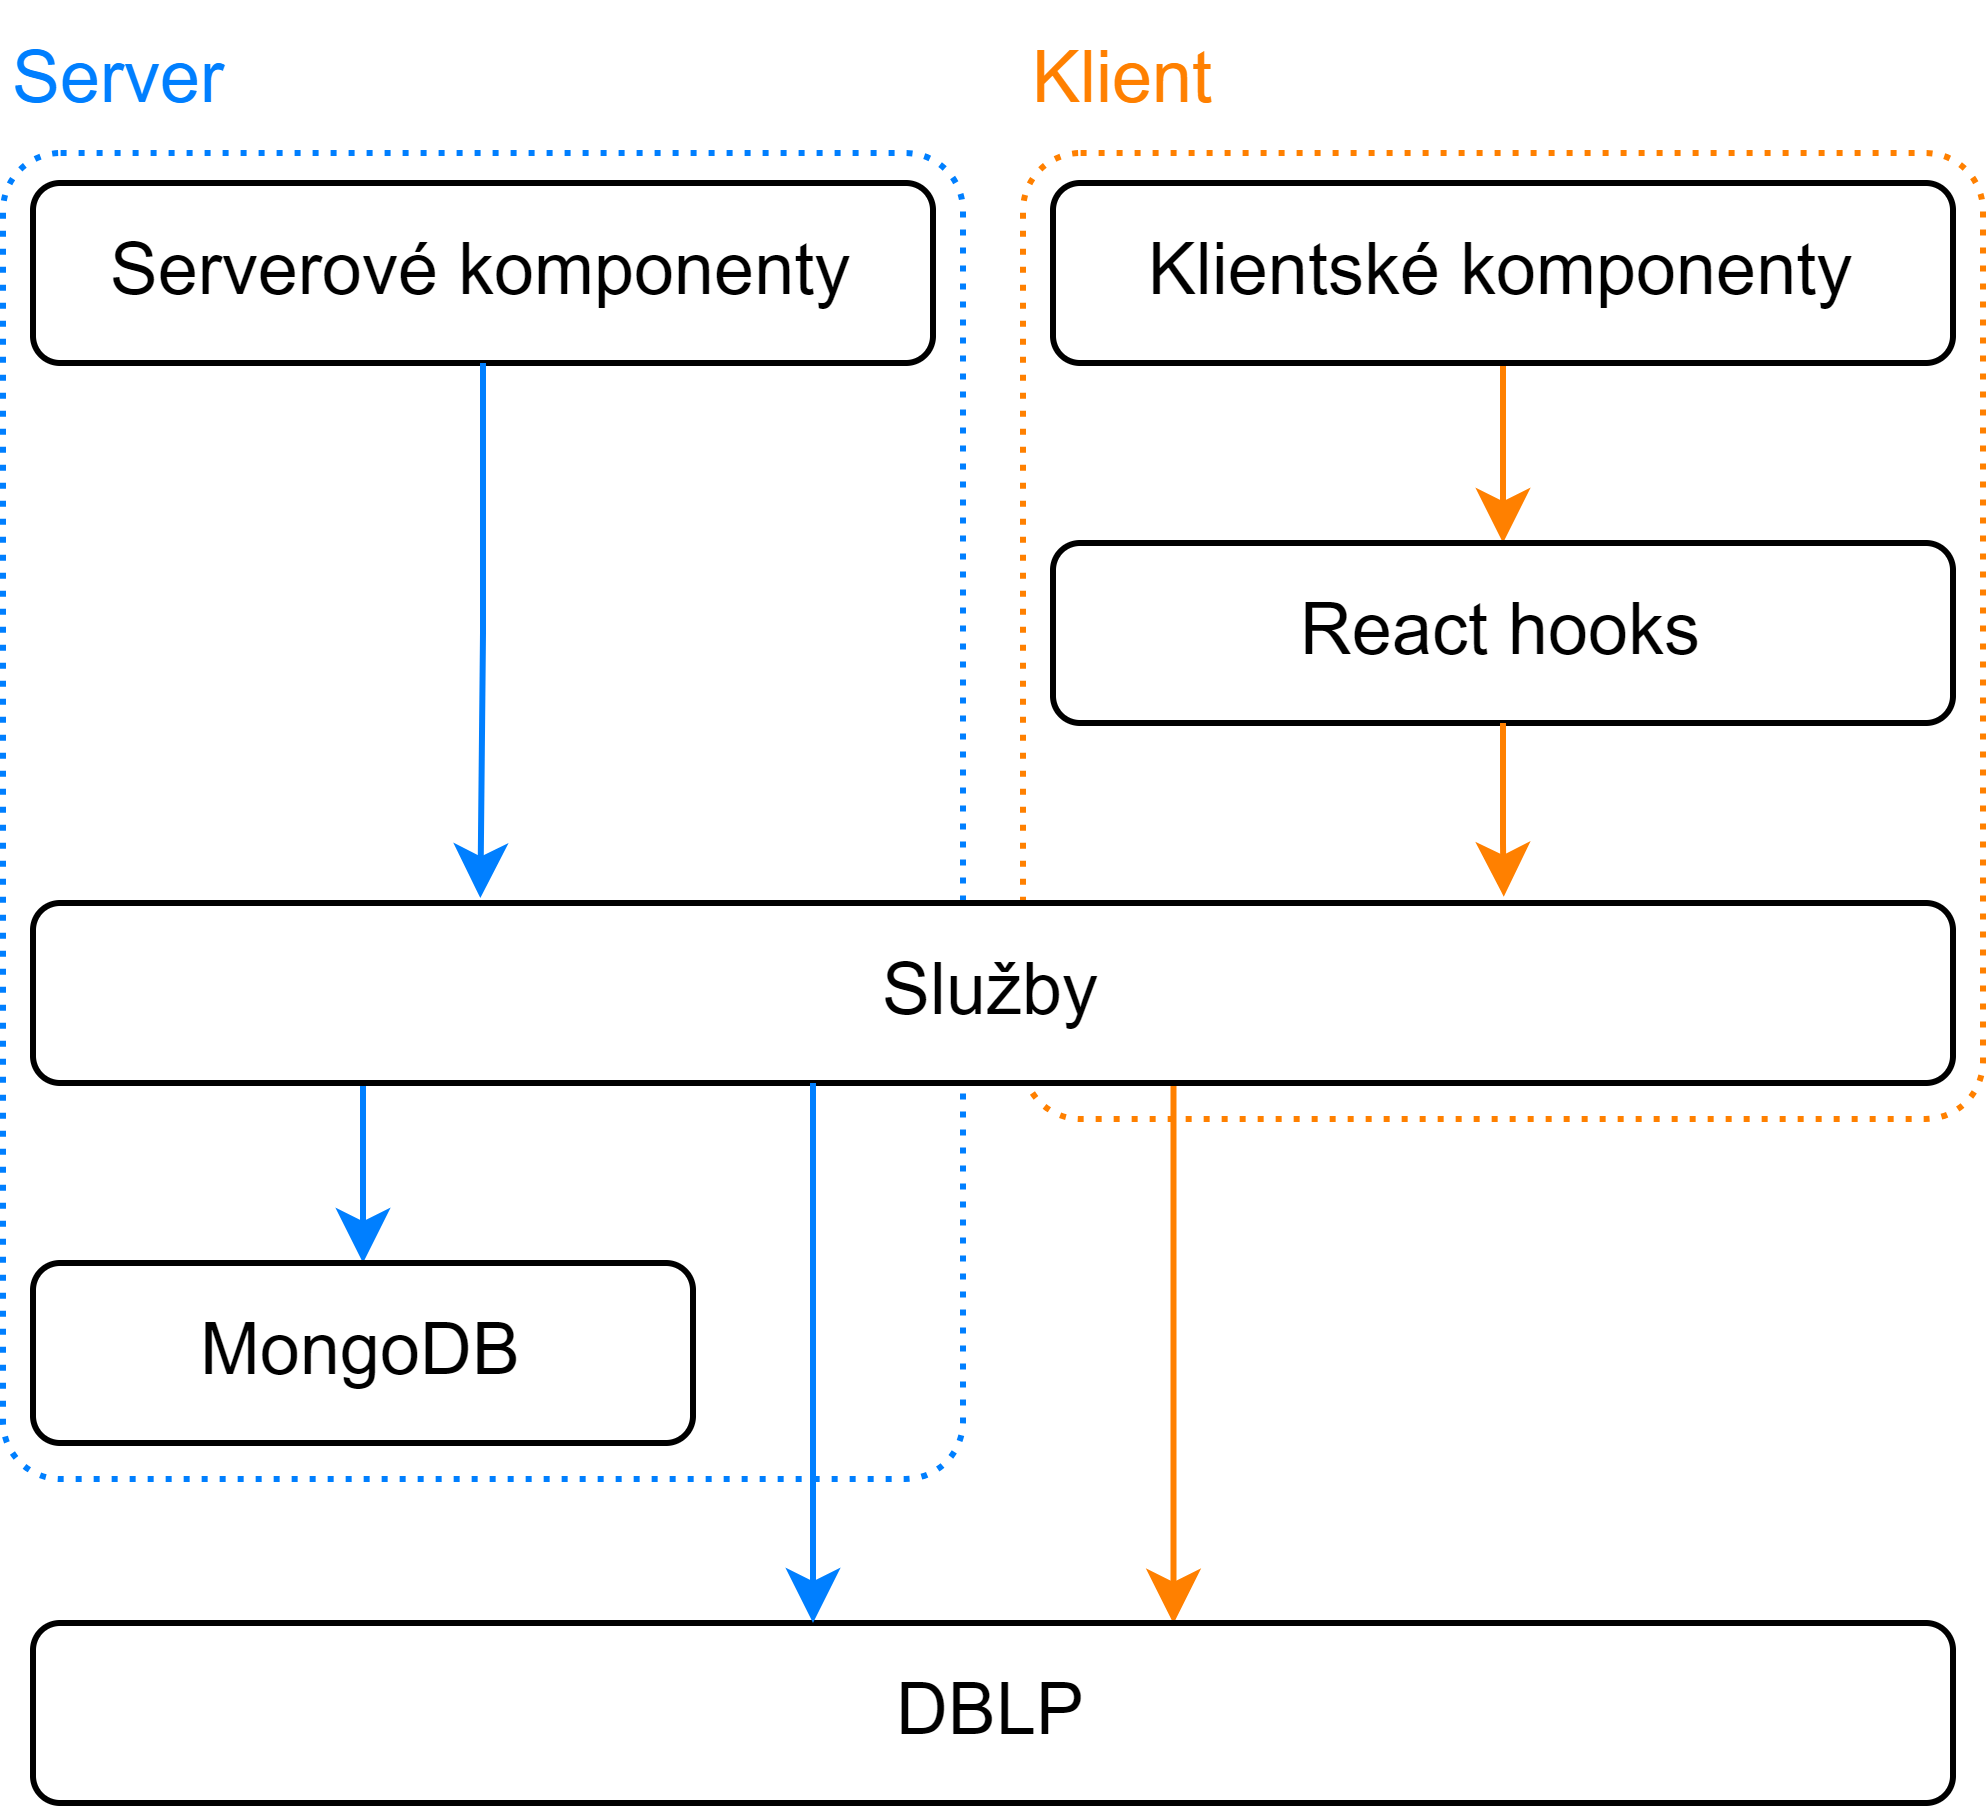
\includegraphics[width=12cm]{architektura_aplikace}
\caption{Architektura aplikace a~znázornění komunikace mezi jejími částmi}\label{fig:architektura_aplikace}
\end{center}
\end{figure}

\subsection{Datová vrstva}

DBLP databáze představuje v~této aplikaci primární zdroj dat. Poskytuje informace o~prezentovaných autorech a proudech publikací. Na tuto databázi se posílají dotazy primárně ze serverové části aplikace, aby mohly být získané záznamy ukládány do mezipaměti. Vlastní řešení mezipaměti jsem implementoval pomocí databázového systému MongoDB. K MongoDB přistupuji skrze modely definované pomocí knihovny Mongoose.

Na straně klienta se posílají dotazy na DBLP databázi pouze pro implementaci rychlého vyhledávání, a~to pomocí \texttt{fetch} API prohlížeče. Konkrétně zde využívám vyhledávacího API, které DBLP poskytuje. Výsledky vyhledávání z~tohoto API aplikace přijímá ve formátu JSON.

\subsection{Prezentační vrstva}

Prezentační vrstvu aplikace tvoří React komponenty, které jsou definované jako funkce. V~Next.js se ve výchozím stavu všechny komponenty renderují na serveru a~klientovi se posílá již vyrenderovaný HTML kód. Tyto komponenty se označují jako \textit{serverové~komponenty}. Příklad serverové~komponenty můžeme vidět na ukázce kódu~\ref{kod:komponenta_SearchAuthorPage}.

\begin{kicode}{JavaScript}{kod:komponenta_SearchAuthorPage}{Serverová komponenta stránky, která na základě parametrů URL adresy načte výsledky vyhledávání autorů a předá je další komponentě pro jejich zobrazení.} [h]
export default async function SearchAuthorPage(
    { searchParams }: SearchAuthorPageParams
) {
    const params = searchToItemsParams(
        searchParams,
        DEFAULT_ITEMS_COUNT_PER_PAGE);
    const result = await getSearchResult(params);

    return (
        <SearchResultList
            result={result}
            searchParams={searchParams}
            paginationUrl={SEARCH_AUTHOR} />
    )
}
\end{kicode}

Serverové komponenty však nemohou být interaktivní a~volat JavaScript na straně klienta. K tomu slouží \textit{klientské~komponenty}, které se renderují až na klientovi. Tyto komponenty definujeme v~souborech anotovaných řetězcem \texttt{use client}. Všechny komponenty, které jsou potomky klientských komponent, jsou opět klientské komponenty.

V aplikaci používám serverové komponenty v~co nejvyšší míře. Tím, že se komponenty renderují již na serveru, se snižuje množství poslaného JavaScript kódu a~kódu, který se musí vykonat na klientovi. Zároveň, pokud je to možné, řeším načítání a~zpracování dat již v~serverových komponentách, abych snížil množství vykonaných HTTP požadavků. Takto načtená data lze předat do klientské komponenty jako běžnou vlastnost React komponenty. Next.js vyřeší přenos dat ze serveru do komponenty automaticky. Klientské komponenty používám kdykoliv, když potřebuji, aby byly schopné reagovat na vstup uživatele nebo pracovat s~API prohlížeče.

\subsection{Aplikační vrstva}

Aplikační vrstvu tvoří primárně služby (services) a~React hooks. Jako \textit{služby} označuji sady funkcí, které poskytují nějakou ucelenou funkcionalitu, typicky zpracování dat. Příkladem může být sada funkcí, která řeší načítání metadat autorů z~DBLP a~jejich následné zpracování pro další použití v~aplikaci.

React hooks implementují logiku aplikace na straně klienta. React komponenty jejich prostřednictvím přistupují k~funkcionalitám služeb. React hooks buď volají služby přímo (například služba pro generování grafu spoluautorství), anebo skrze HTTP koncový bod, pokud daná služba musí být vykonána na straně serveru (například stažení metadat autora). Ve~druhém případě využívám \texttt{fetch}~API a~knihovnu~SWR. Příkladem takového React hook je funkce \texttt{useAuthor}, jejíž definici můžeme vidět na ukázce kódu~\ref{kod:useAuthor_hook}.

\begin{kicode}{JavaScript}{kod:useAuthor_hook}{React hook \texttt{useAuthor}, který umožňuje prostřednictvím knihovny SWR stáhnout metadata autora ze serveru.} [h]
export default function useAuthor(authorId: string) {
    const { data, error, isLoading } = useSWRImmutable(
        authorId,
        authorFetcher);

    return {
        author: data,
        isLoading,
        error
    };
}

async function authorFetcher(authorId: string) {
    await waitForNextFetchClient();
    const response = await fetch("/api/author/" + authorId);
    return await response.json() as DblpAuthor;
}
\end{kicode}

Dále React hooks používám čistě jen pro oddělení logiky React komponenty od její vizualizace. Výsledkem je lepší znovupoužitelnost a~čitelnost kódu.

\newpage

\subsection{Organizace kódu}

Kód aplikace je rozdělen do funkcí, které jsou dále podle poskytované funkcionality rozděleny do souborů. Pokud je funkce z~jednoho souboru potřeba v~jiném souboru, je vyexportovaná do JavaScript modulu. Soubory jsou nakonec rozdělené podle účelu do adresářů. Všechen kód aplikace nalezneme v~adresáři \texttt{src/}, který obsahuje konfigurační soubory použitých knihoven a následující adresáře:

\begin{itemize}
\item \texttt{\_\_tests\_\_/} -- Adresář s~jednotkovými testy napsanými pomocí knihovny Jest. Pokrytí kódu automatizovanými testy je jedním z~nedostatků aplikace. Jednotkovými testy jsou zatím pokryty pouze utility funkce.
\item \texttt{app/} -- Stěžejní adresář Next.js aplikace, která využívá App Router. Obsah tohoto adresáře popisuje mapování segmentů URL adres na stránky aplikace. Ty jsou tvořeny React komponentami umístěnými v~souborech s~názvem page.tsx.
\item \texttt{components/} -- Adresář se všemi React komponentami, které jsou sdílené mezi více stránkami.
\item \texttt{constants/} -- Adresář s~konstantami. Některé konstanty, které se používají pouze v~rámci jednoho souboru, zde nemusí být zahrnuty.
\item \texttt{css/} -- Adresář s~CSS soubory, ve kterých najdeme například definované barevné téma aplikace nebo vizualizaci tlačítek.
\item \texttt{db/} -- Adresář s~definicí schémat MongoDB databáze a~modelů, pomocí kterých lze přistupovat k~datům databáze. V~souboru \texttt{mongodb.ts} se nachází stěžejní funkce \texttt{connectDb} pro vytvoření spojení s~databází. Je~nutné ji volat před přístupem k~databázi.
\item \texttt{dtos/} -- Adresář s~TypeScript typy pro objekty, které se používají k~výměně dat mezi různými částmi aplikace.
\item \texttt{enums/} -- Adresář s~výčtovými typy.
\item \texttt{hooks/} -- Adresář s~React hooks. Některé React hooks, které se používají pouze v~rámci jednoho souboru (respektive React komponenty), zde nemusí být zahrnuty.
\item \texttt{public/} -- Adresář se statickým obsahem, který je přístupný z~klienta.
\item \texttt{services/} -- Adresář se všemi službami aplikace.
\item \texttt{utils/} -- Adresář s~\textit{utility~funkcemi}, tedy jednoúčelovými pomocnými funkcemi. Najdeme zde například pomocné funkce pro práci s~řetězci, poli nebo URL adresami.
\end{itemize}

\subsection{Stránky a~API aplikace}

Na~obrázku~\ref{fig:struktura_url_adres_stranek_aplikace} můžeme vidět znázorněnu organizaci všech stránek aplikace z~pohledu jejich URL adres. Aplikace nabízí následující stránky:

\begin{itemize}
\item Úvodní stránka -- Obsahuje jednoduchý rozcestník na stránky indexů autorů a~proudů publikací.
\item Stránka autora -- Obsahuje vizualizace různých statistik autora a~interaktivní graf jeho spoluautorů.
\item Stránka s~publikacemi autora -- Obsahuje přehled publikací autora s~možností jejich filtrování.
\item Stránka skupiny autorů -- Obsahuje vizualizace různých statistik skupiny autorů, kterou si uživatel vytvořil, a~interaktivní graf jejich spoluautorů.
\item Stránka s~publikacemi skupiny autorů -- Obsahuje přehled publikací skupiny autorů s~možností jejich filtrování.
\item Stránka proudu publikací -- Obsahuje vizualizace různých statistik proudu publikací a~přehled případných svazků daného proudu publikací. V~případě existence svazků umožňuje jejich výběr a~zobrazení vizualizací různých jejich statistik a~interaktivního grafu autorů publikací z~vybraných svazků.
\item Stránka s~publikacemi proudu publikací -- Obsahuje přehled publikací proudu publikací s~možností jejich filtrování. V případě existence svazků umožňuje jejich výběr a~zobrazení přehledu jejich publikací.
\item Stránka svazku -- Obsahuje vizualizace různých statistik svazku a~interaktivní graf autorů jeho publikací.
\item Stránka s~publikacemi svazku -- Obsahuje přehled publikací svazku s~možností jejich filtrování.
\item Stránka s~indexem autorů nebo výsledky jejich vyhledávání.
\item Stránka s~indexem proudů publikací nebo výsledky jejich vyhledávání.
\end{itemize}

Aplikace taktéž nabízí koncový bod API, který uživatele podle zadaného jména přesměruje buď na stránku autora tohoto jména, pokud v~DBLP databázi existuje pouze jeden autor daného jména, nebo na stránku s~výsledky vyhledávání autorů daného jména. Tento koncový bod se využívá v~situacích, kdy není k~dispozici unikátní identifikátor autora, ale jen jeho jméno.

\begin{figure}[H]
\begin{center}
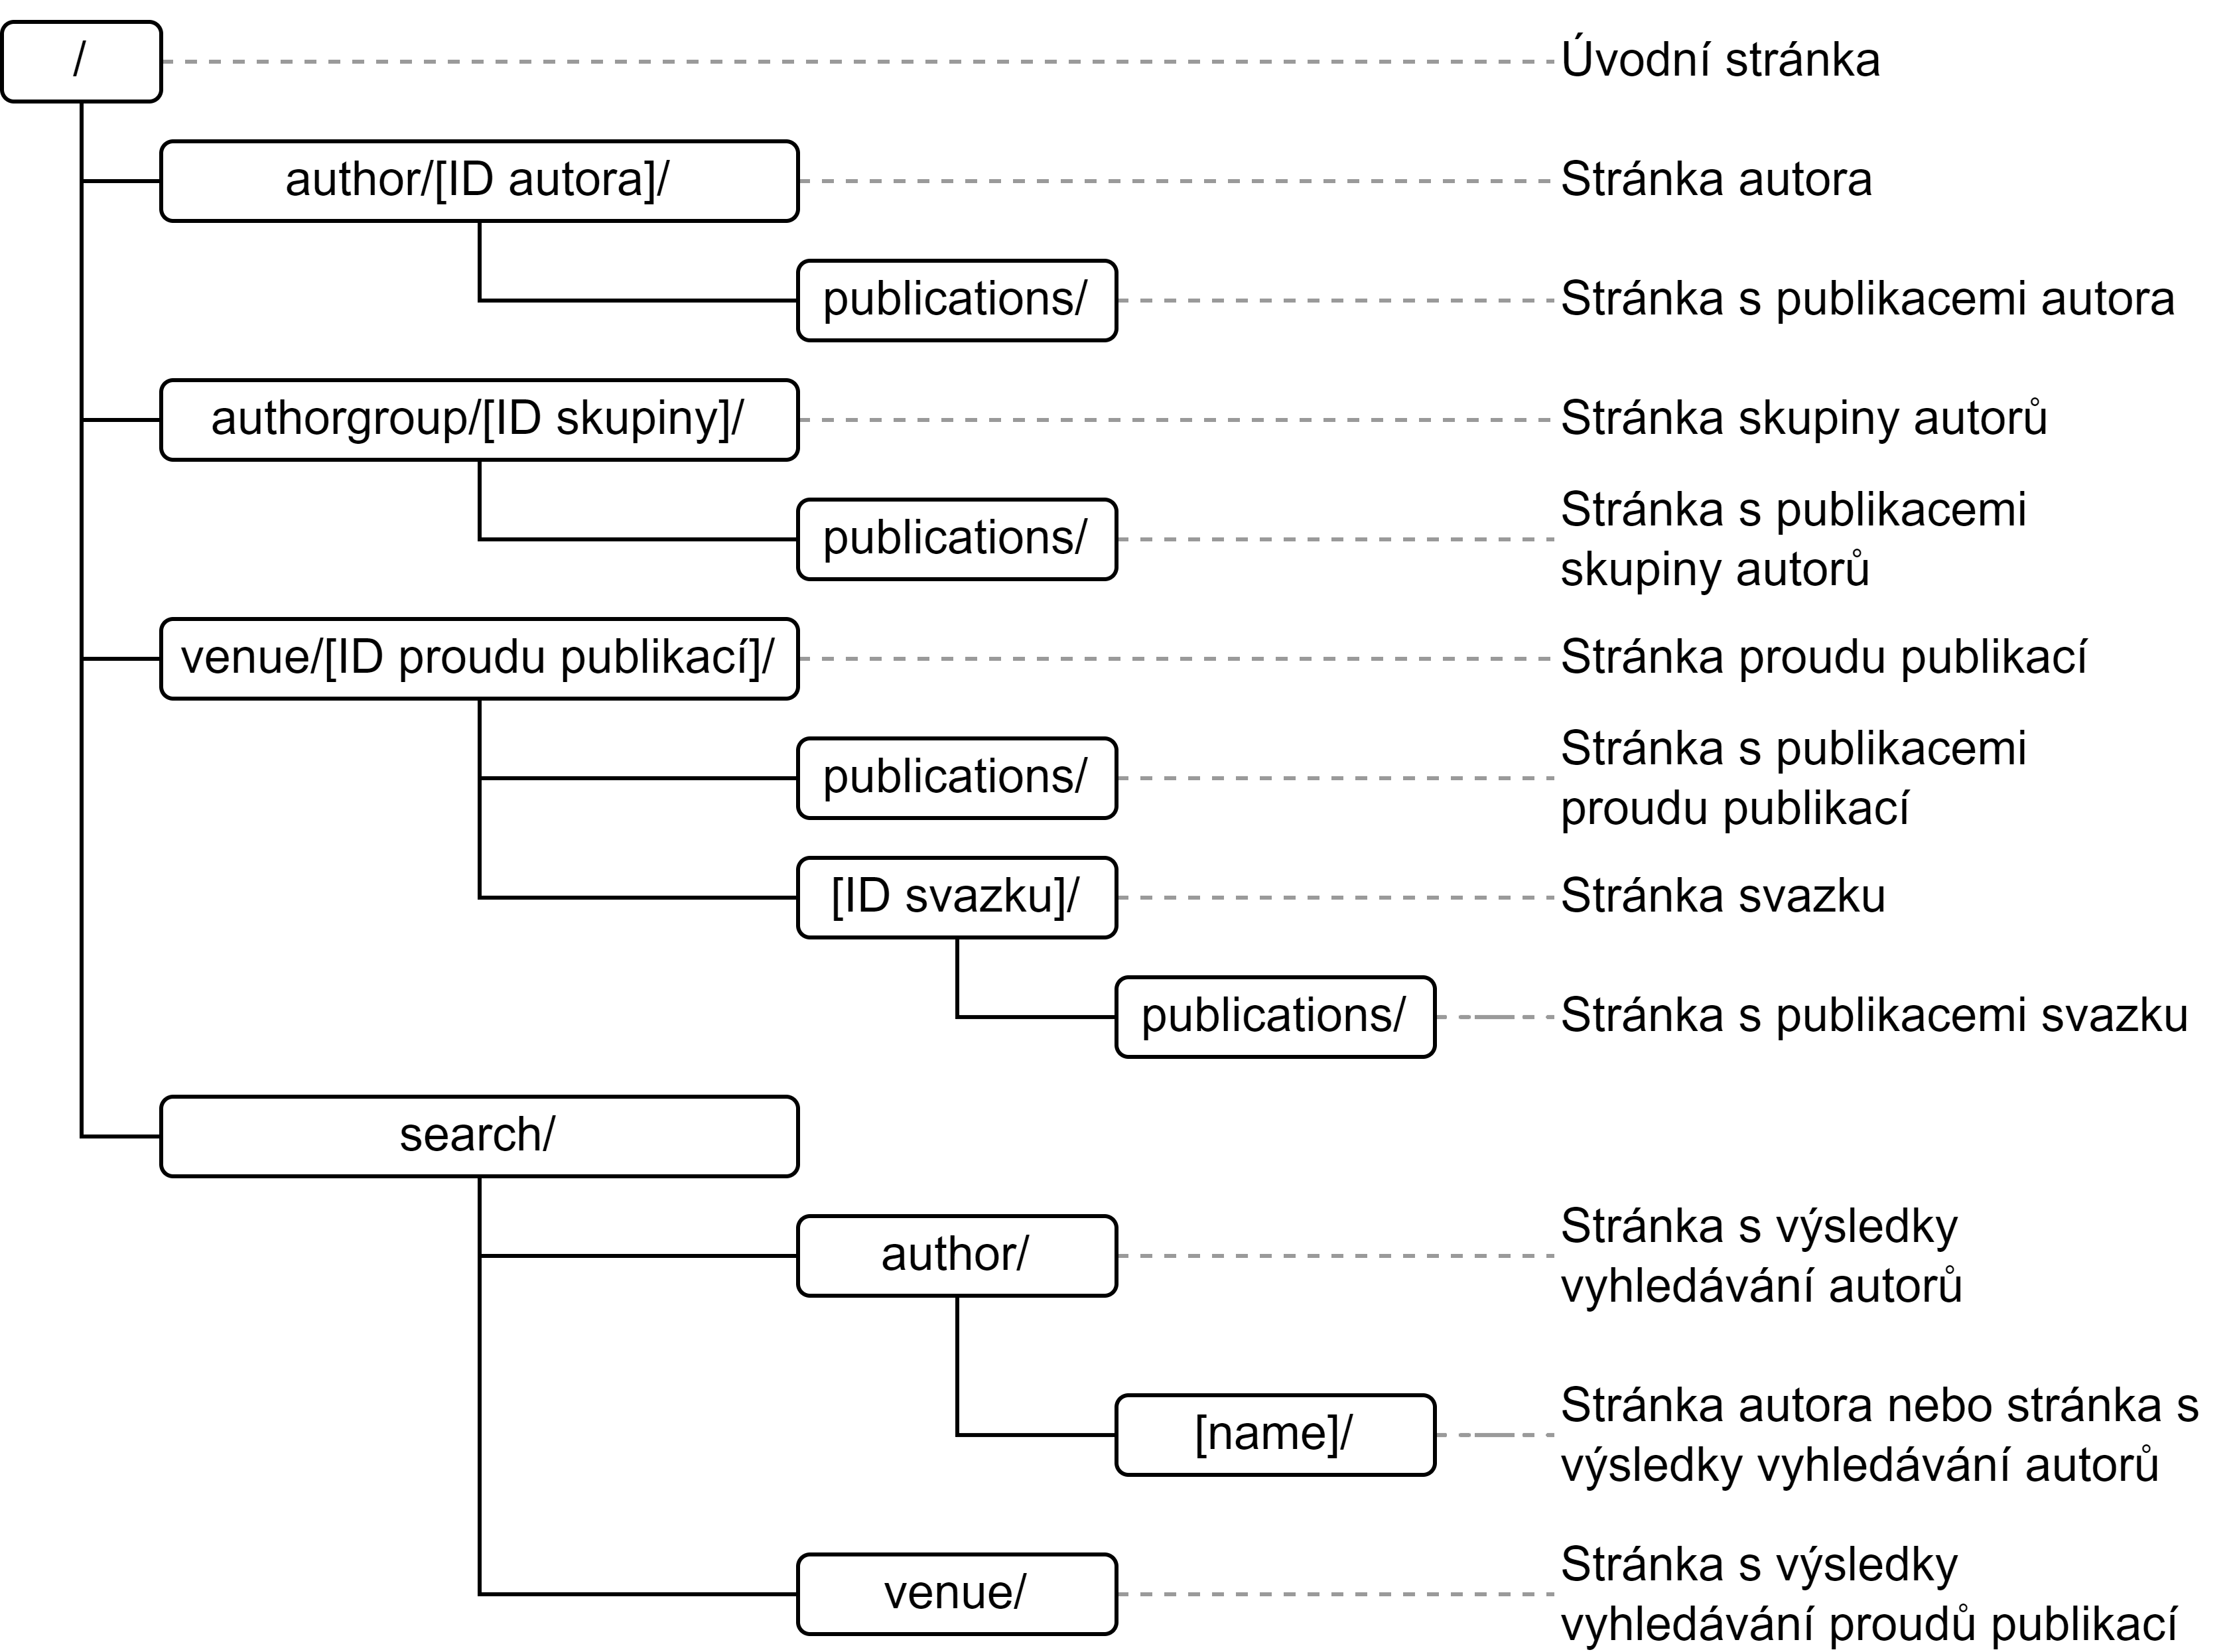
\includegraphics[width=\textwidth]{urls_lokalnich_stranek}
\caption{Organizace stránek aplikace z~pohledu jejich URL adres}\label{fig:struktura_url_adres_stranek_aplikace}
\end{center}
\end{figure}

Dále API aplikace poskytuje ještě tři koncové body, jejichž URL adresy můžeme vidět na obrázku~\ref{fig:struktura_url_adres_api_aplikace}:
\begin{itemize}
\item koncový bod vracející metadata autora s~předaným identifikátorem,
\item koncový bod vracející metadata autorů s~předanými identifikátory,
\item koncový bod vracející metadata proudu publikací nebo svazku s~předaným identifikátorem.
\end{itemize}

\begin{figure}[H]
\begin{center}
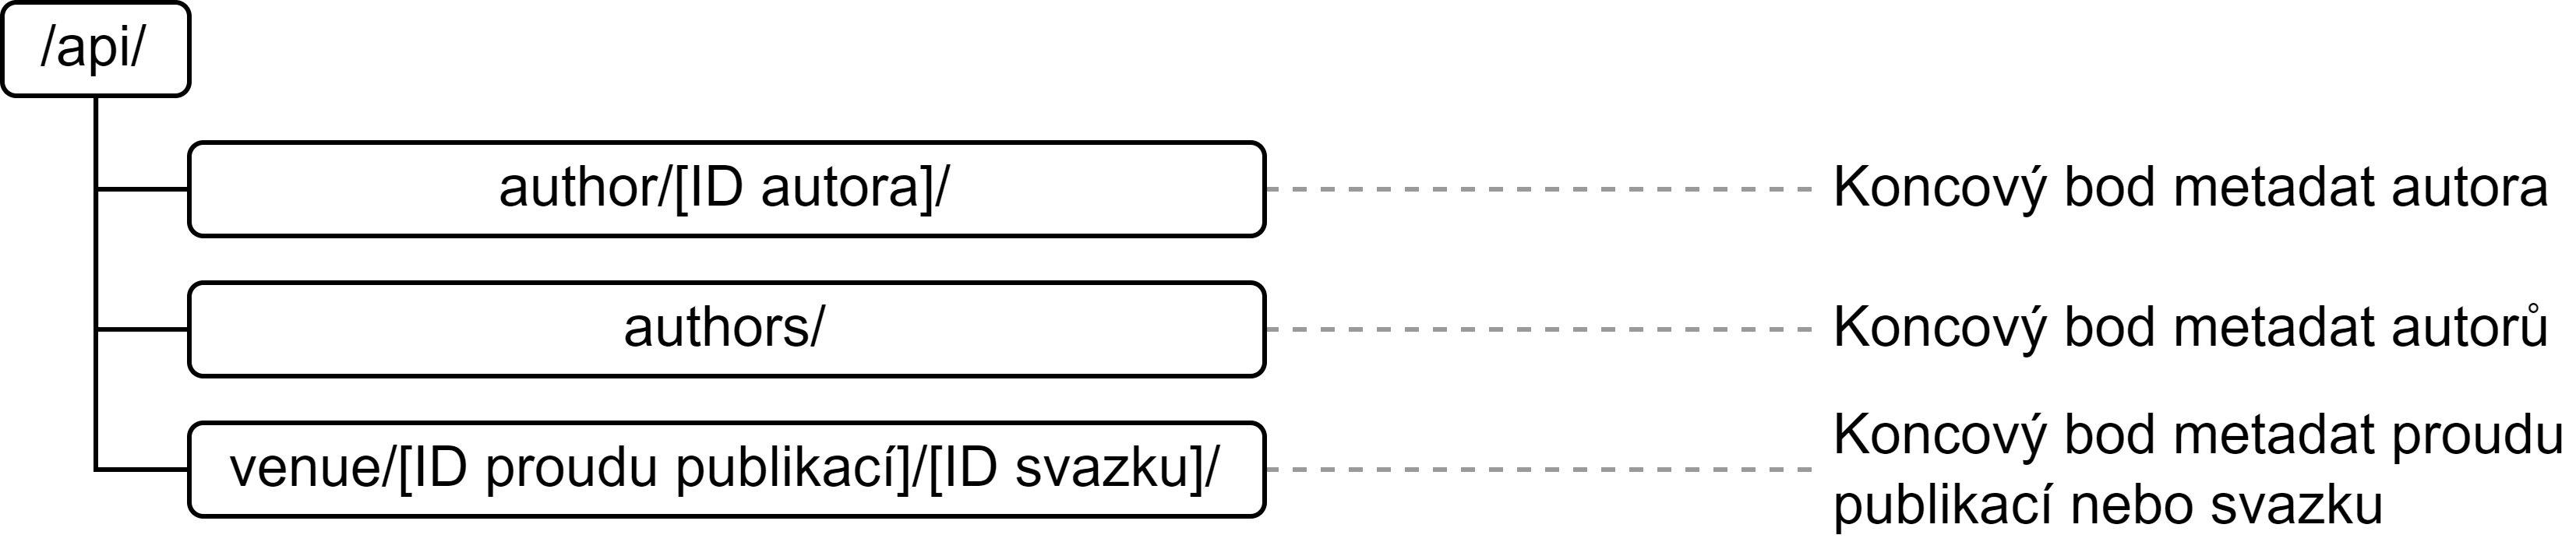
\includegraphics[width=\textwidth]{urls_lokalniho_api}
\caption{URL adresy koncových bodů API aplikace}\label{fig:struktura_url_adres_api_aplikace}
\end{center}
\end{figure}

\newpage

\section{Práce s daty}

%% popsat, které služby řeší stahování?

Z~možností stažení dat z~DBLP, jejichž přehled najdeme v~kapitole~\ref{sec:moznosti_stazeni_dat}, jsem se rozhodl využít následující:

\begin{itemize}
\item stažení stránek ve formátu HTML -- pro získání indexů autorů a~proudů publikací,
\item stažení stránek ve formátu XML -- pro získání metadat autorů, proudů publikací a~svazků,
\item API pro vyhledávání -- pro implementaci vyhledávání autorů a~proudů publikací.
\end{itemize}

Jednodušší implementace těchto možností podle mého názoru převažuje výhody použití celého datasetu v~podobě souboru \texttt{dblp.xml}. Především nemusím řešit pravidelné obnovování datasetu a uživatel tak má vždy zajištěn přístup k~aktuálním datům. Taktéž nemusím řešit vlastní implementaci vyhledávání.

\begin{figure}[H]
\begin{center}
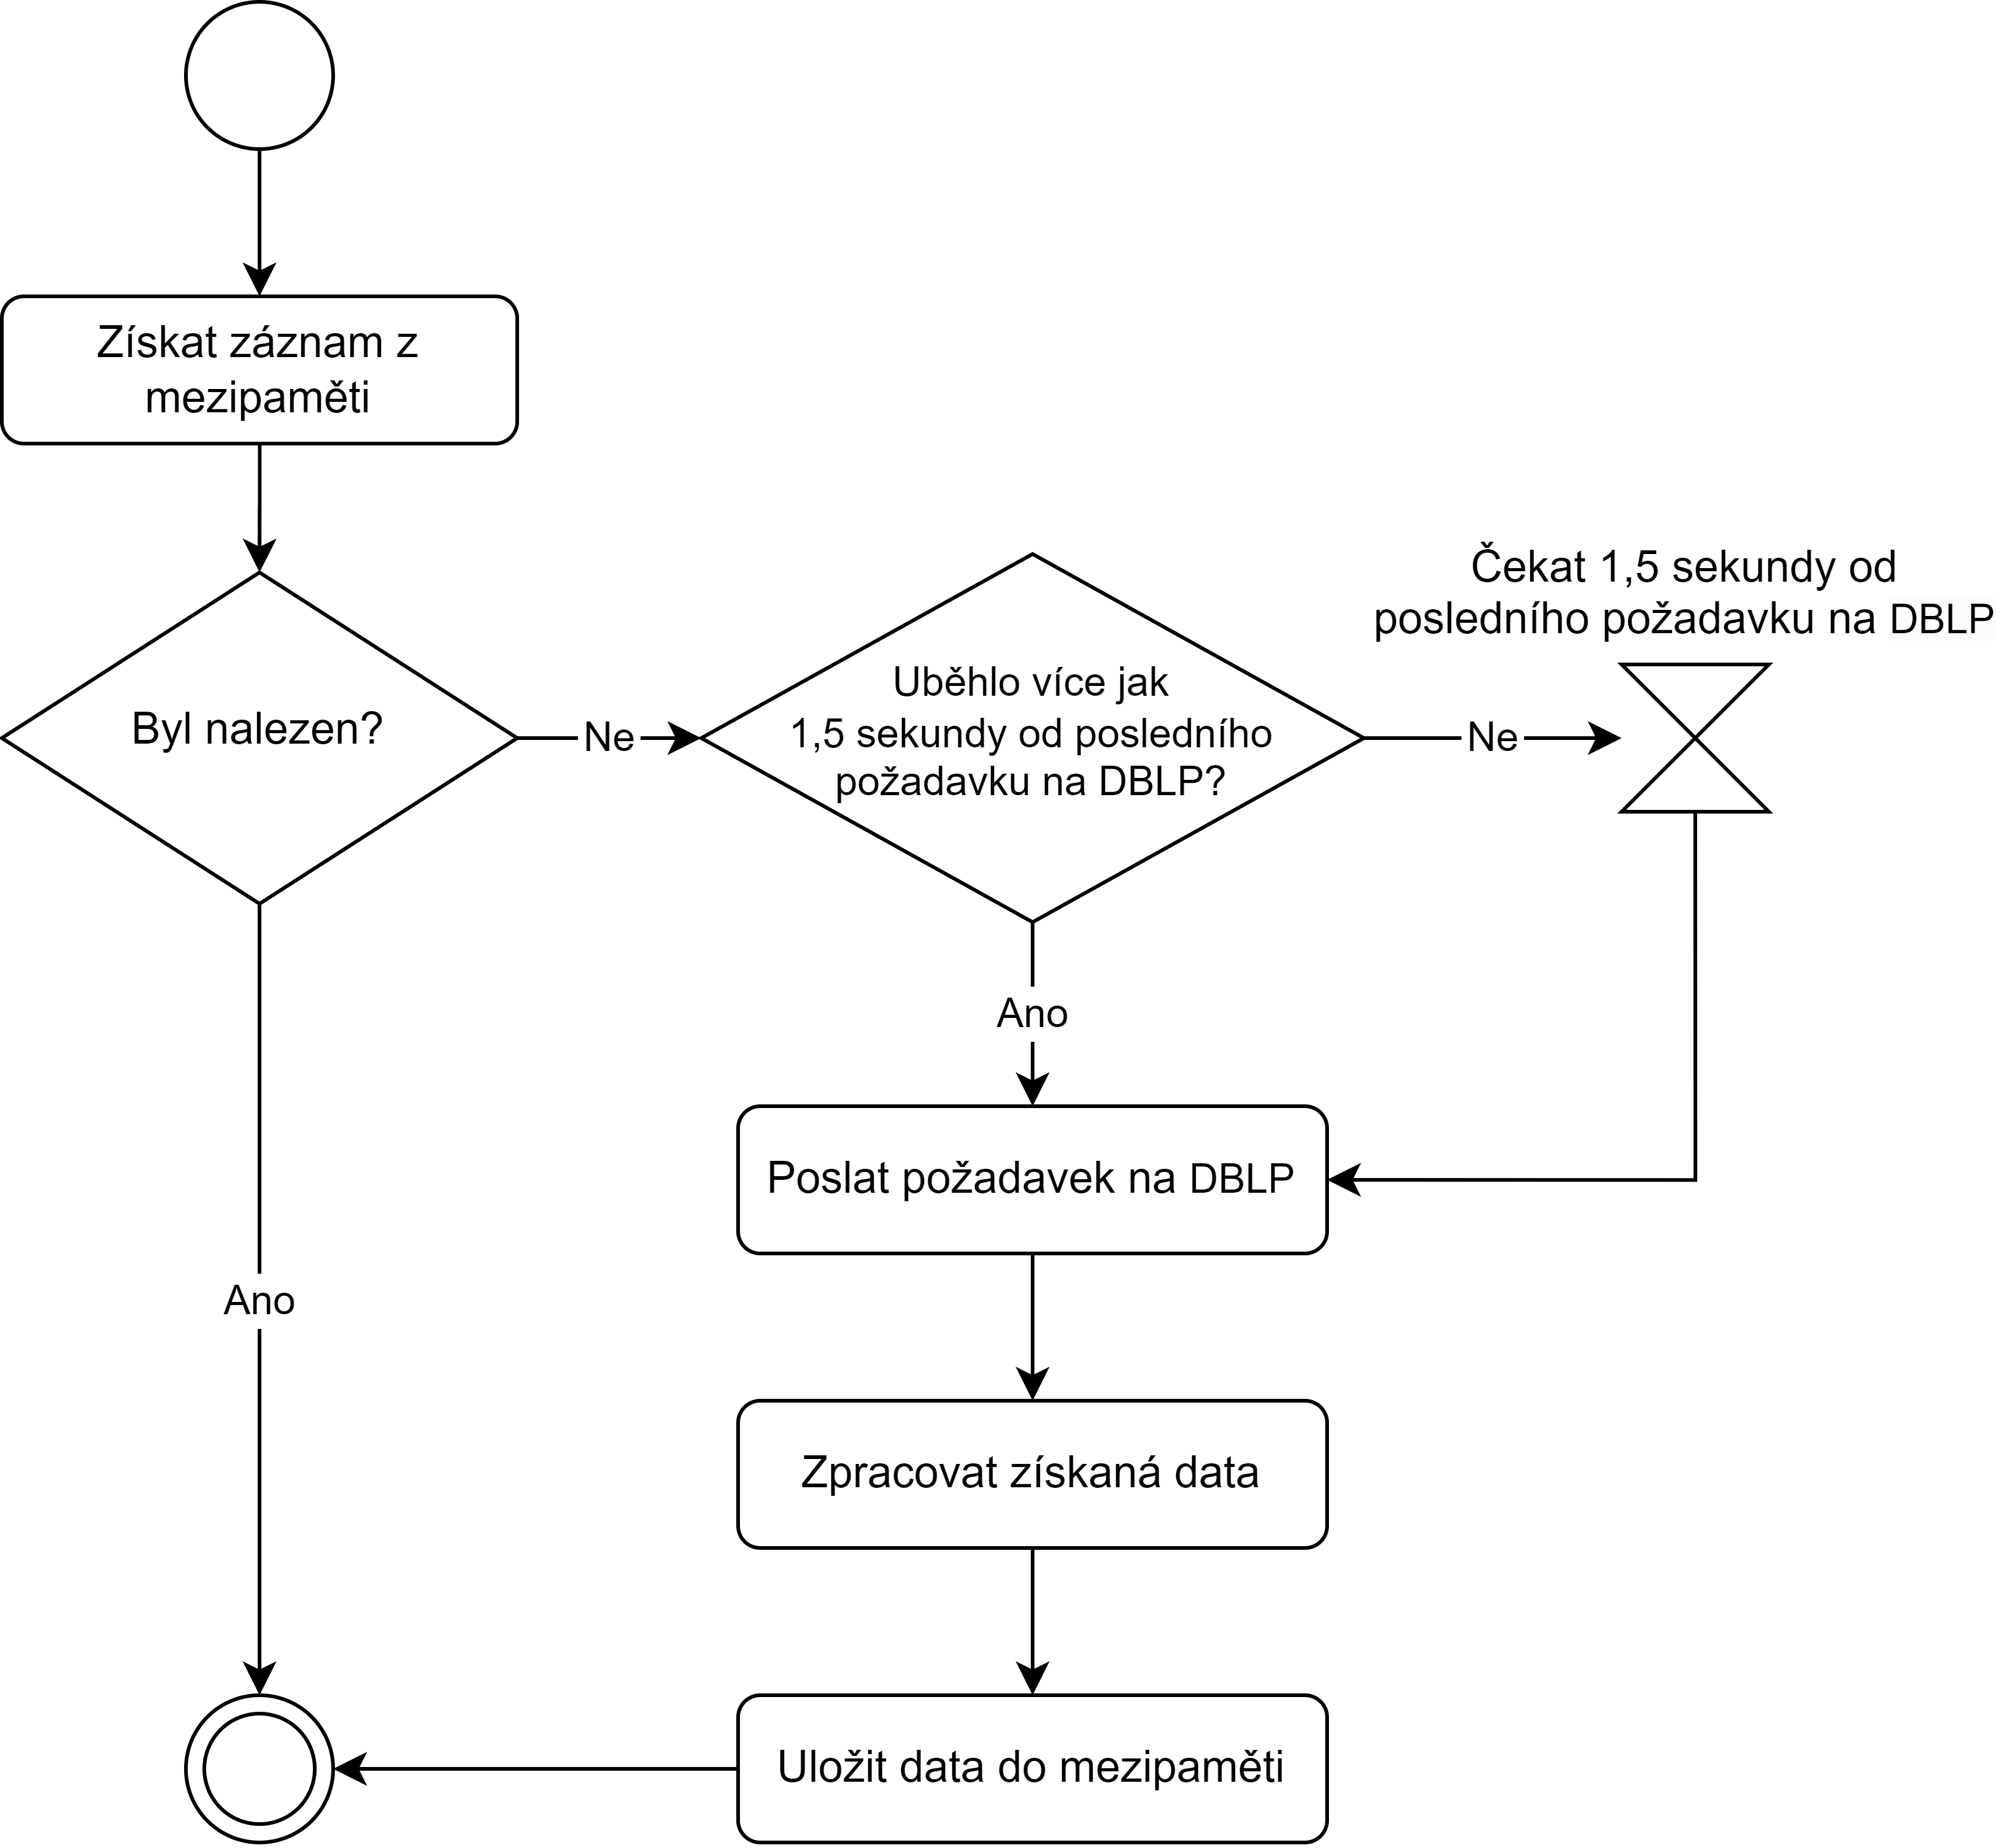
\includegraphics[width=13.4cm]{nacitani_dat}
\caption{Diagram aktivit popisující načítání metadat autora, proudu publikací nebo svazku}\label{fig:nacitani_dat}
\end{center}
\end{figure}

Aby nedocházelo k~přetížení služby, doporučují autoři DBLP čekat mezi dvěma po sobě následujícími požadavky alespoň jednu nebo dvě sekundy. Já se v~situacích, kdy by potenciálně mohlo docházet k~odeslání většího množství požadavků v~kratším časovém intervalu, rozhodl čekat mezi požadavky alespoň 1,5~sekundy. Toto čekání zajišťuje asynchronní funkce \texttt{waitForNextFetch}, která se volá před odesláním požadavku na~DBLP. Funkce si do databáze ukládá čas poslání posledního požadavku na DBLP. Pokud při volání této funkce uběhlo méně než 1,5~sekundy od poslání posledního požadavku na DBLP, funkce čeká dostatečně dlouhou dobu, aby tomu tak bylo.

Problém přetížení DBLP zasláním většího množství požadavků dále řeším využitím mezipaměti. Využívám jak zcela automatické řešení v~Next.js a~knihovně SWR, tak i~vlastní řešení postavené na databázovém systému MongoDB. Vlastní řešení mezipaměti používám pouze u~záznamů získaných ze stránek ve formátu XML. Tyto stránky totiž někdy přesahují velikost 2~MB a~mezipaměť poskytovaná frameworkem Next.js neumožňuje uložení záznamů, jejichž velikost přesahuje~2~MB. Popis procesu získání metadat ze stránek ve formátu XML můžeme vidět na obrázku~\ref{fig:nacitani_dat}.

\subsection{Vlastní identifikátory}

V~rámci aplikace jsem se rozhodl používat vlastní identifikátory autorů, proudů publikací a~svazků. Jejich identifikátory v~DBLP totiž mohou obsahovat znak \uv{/}. Protože však potřebuji identifikátory předávat přes URL adresu a~znak~\uv{/} v~identifikátoru by tento proces komplikoval, nahrazuji v~každém identifikátoru všechny znaky~\uv{/} posloupností dvou znaků~\uv{\_}. Například namísto identifikátoru \uv{journals/aiopen} tak pracuji s~identifikátorem \uv{journals\_\_aiopen}.

\subsection{Zpracování stažených dat}

Extrahování dat ze souborů ve formátu HTML nebo XML na straně serveru řeším pomocí knihovny Cheerio. Funkce provádějící tuto extrakci se nacházejí v~souborech:

\begin{itemize}
\item \texttt{src/services/authors/parsing.ts} -- obsahuje funkce pro extrahování indexu autorů a~metadat autorů,
\item \texttt{src/services/venues/parsing.ts} -- obsahuje funkce pro extrahování indexu proudů publikací a~metadat proudů publikací a~svazků,
\item \texttt{src/services/publications/parsing.ts} -- obsahuje funkce pro extrahování metadat publikací, které jsou sdílené předchozími soubory.
\end{itemize}

Nejkomplikovanější je extrahování metadat ze stránek proudů publikací ve formátu XML. Tyto stránky totiž nemají pevně danou strukturu a~kombinují standardní HTML značky se značkami vlastními. V~některých případech jsou odkazy na svazky umístěné například v~tabulce \texttt{<table>} a~v~jiných zase v~seznamech \texttt{<ul>}, které mohou být do sebe i~několikanásobně zanořené. Dále jsou v~mnoha případech metadata publikací uvedena již na stránce proudu publikací. Takové publikace většinou samy reprezentují stránky svazků a~slouží jako odkazy na ně. Taktéž se může jednat o~proudy publikací, které se již dále nedělí na svazky.

Výstupem funkcí pro extrahování metadat jsou objekty sloužící k~výměně dat mezi různými částmi aplikace. Jejich TypeScript typy a~funkce pro jejich vytvoření se nachází v~adresáři \texttt{src/dtos/}. Stěžejní typy jsou následující:
\begin{itemize}
\item \texttt{DblpPublication} -- pro metadata publikace,
\item \texttt{DblpAuthor} -- pro metadata autora,
\item \texttt{DblpVenue} -- pro metadata proudu publikací,
\item \texttt{DblpVenueVolume} -- pro metadata svazku,
\item \texttt{SimpleSearchResult} -- pro indexy a~výsledky vyhledávání autorů nebo proudů publikací.
\end{itemize}

%% třídní diagramy stěžejních DTO?

\subsection{Data uživatele}

Data uživatele se ukládají do úložiště prohlížeče \texttt{localStorage}. Konkrétně se jedná o~následující data:
\begin{itemize}
\item naposledy navštívení autoři,
\item naposledy navštívené proudy publikací nebo svazky,
\item uložení autoři pro snazší přístup,
\item uložené proudy publikací nebo svazky pro snazší přístup,
\item vytvořené skupiny autorů.
\end{itemize}

Nevýhodou tohoto řešení je, že uživatel nemá takto uložená data snadno přístupná z~různých prohlížečů. Proto jsem zvažoval i~možnost uložení dat uživatele v~databázi na straně serveru. Toto řešení by vyžadovalo implementaci autentizace a~autorizace uživatele, aby měl přístup jen ke svým datům, což by však zkomplikovalo návrh celé aplikace. Nutnost registrace by navíc mohla odradit některé uživatele od používání aplikace. Nakonec jsem se tak rozhodl ukládat data do úložiště prohlížeče a~přidal do aplikace možnost exportu a~importu dat uživatele.

Do \texttt{localStorage} se z~důvodu omezené velikosti neukládají celé objekty autorů, proudů publikací a~svazků, ale jen jich identifikátory a~názvy. Zbylá metadata se stahují voláním koncových bodů API aplikace.

\newpage

\section{Klíčové komponenty aplikace}

Aplikace obsahuje řadu základních univerzálních komponent. Jedná se například o~různá tlačítka, kontejnery, záložky, tabulky nebo dialogy. Jejich kombinací vznikají komponenty složitější. Z~nich jsou klíčové především komponenty pro vizualizaci statistik a~komponenta grafu spoluautorství. Aplikace nepoužívá kromě Next.js žádnou další knihovnu poskytující již hotové React komponenty.

\subsection{Vizualizace statistik}

Většina statistik, které aplikace umožňuje vizualizovat, jsou kolekce párů typu \uv{klíč--číselná hodnota}. Například statistika udávající počty zveřejněných publikací v~jednotlivých letech. Aplikace nabízí celkem tři React komponenty pro vizualizaci takových kolekcí:
\begin{itemize}
\item \texttt{LineChart} -- liniový graf,
\item \texttt{BarChart} -- sloupcový graf,
\item \texttt{PieChart} -- koláčový graf.
\end{itemize}

Komponenty na vstup dostávají seznam položek, které seskupí podle zkoumané vlastnosti a~každé skupině přiřadí číselnou hodnotu. Tím vzniká kolekce párů typu \uv{klíč--číselná hodnota}, kde klíčem je hodnota zkoumané vlastnosti. Tuto kolekci komponenta vizualizuje formou požadovaného grafu.

Vstupní data, která chceme vizualizovat, jsou komponentám předávána jako objekt typu \texttt{ChartData}. Každá komponenta si tento typ rozšiřuje o~vlastní vlastnosti. Typ \texttt{ChartData} definuje především vlastnosti pro:
\begin{itemize}
\item seznam zkoumaných položek (například seznam publikací autora),
\item funkci, která pro předanou položku vrací hodnotu zkoumané vlastnosti,
\item funkci, která předané skupině přiřazuje číselnou hodnotu (pokud není definovaná, volí se počet položek skupiny).
\end{itemize}

Samotné grafy tvoří kombinace SVG a~HTML elementů. Mapování dat na různé typy vizuálních hodnot, měřítek nebo os zajišťuje knihovna D3.js. Nevyužívám však možnosti manipulace s~DOM, kterou tato knihovna poskytuje. Manipulace s~DOM je zcela v~režii knihovny React.

Grafy a~tabulky prezentující konkrétní statistiku se vždy sdružují do jedné komponenty, která umožňuje mezi různými prezentacemi přepínat. Příkladem může být komponenta \texttt{PublicationsOverTimeStats} pro statistiku udávající počty zveřejněných publikací v~jednotlivých letech. Komponenty všech statistik najdeme v~adresáři \texttt{components/data-visualsation/stats/}.

\subsection{Graf spoluautorství}

O~vytvoření datových struktur, které reprezentují graf spoluautorství množiny autorů, se stará funkce \texttt{convertToCoauthorsGraph}. Tato funkce přijímá pole publikací, jež převádí na pole uzlů reprezentujících autory a~pole neorientovaných hran mezi těmito uzly. Hrana je vytvořena mezi každými dvěma autory stejné publikace ze vstupního pole. Dále funkce ještě vrací objekt slovníku. Tento slovník mapuje identifikátory autorů na jejich uzly a~umožňuje tak rychlý přístup k~uzlům na základě jejich identifikátorů.

Zobrazení interaktivní vizualizace grafu a~souvisejících informací, jako je například seznam autorů v~grafu nebo informace o~aktuálně vybraném autorovi, zajišťuje React komponenta \texttt{CoauthorsGraphShell}. Stav grafu, se kterým tato komponenta pracuje, spravuje React hook \texttt{useCoauthorsGraph}. Samotný graf se vykresluje na HTML element \texttt{<canvas>}. Určení souřadnic uzlů grafu je založeno na simulaci fyzikálních sil implementované pomocí knihovny D3.js~\cite{t33}. V~simulaci se na uzly grafu aplikují celkem tři síly:
\begin{itemize}
\item \texttt{forceLink} -- přitahuje k~sobě uzly propojené hranou,
\item \texttt{forceManyBody} s~negativní intenzitou -- vzájemně od sebe odpuzuje všechny uzly,
\item \texttt{forceCenter} -- všechny uzly přitahuje do specifikovaného bodu.
\end{itemize}

Jelikož je tato simulace výpočetně náročná, rozhodl jsem se ji vykonávat na pozadí v~rámci pracovního vlákna poskytovaného funkcionalitou Web~Worker~\cite{t34}. Pracovní vlákno přerušuje to hlavní pouze zasíláním průběžného postupu simulace a~konečného výsledku v~podobě pole uzlů a~hran s~aktualizovanými souřadnicemi. Na ukázce kódu \ref{kod:simulace_grafu_spoluautorstvi} můžeme vidět kód pro vytvoření simulace.

\begin{kicode}{JavaScript}{kod:simulace_grafu_spoluautorstvi}{Kód pro vytvoření simulace fyzikálních sil, která určí souřadnice uzlů grafu.} [h]
const simulation = d3.forceSimulation(event.data.nodes)
    .force('link', d3.forceLink()
        .id((d) => d.person.id)
        .links(event.data.links))
    .force('charge', d3.forceManyBody().strength(-50))
    .force('center', d3.forceCenter(
        event.data.graphWidth / 2,
        event.data.graphHeight / 2))
    .stop();
\end{kicode}

\newpage

\section{Zprovoznění aplikace}

Aplikaci je možné zprovoznit dvěma způsoby, a~to buď pomocí Docker, anebo bez něj. První zmiňovaný způsob je určen pro testování a~nasazení produkční verze aplikace. Druhý způsob je pak určen především pro vývoj.

\subsection{Za použití Docker}

Ke zprovoznění aplikace pomocí Docker je potřeba mít nainstalovánu jeho aktuální verzi spolu s~Docker Compose. V~přiložených elektronických datech v adresáři \texttt{src/} jsou k~dispozici dva Docker Compose soubory:

\begin{itemize}
\item \texttt{docker-compose-dev.yml} -- pro lokální testování aplikace v produkčním režimu (aplikace běží na portu 3000),
\item \texttt{docker-compose-prod.yml} -- pro nasazení aplikace na produkci (aplikace běží na portu 80).
\end{itemize}

Oba soubory zajistí vytvoření a~spuštění MongoDB a~samotné aplikace. Potřebné proměnné prostředí a~porty aplikací jsou předdefinované již v~těchto souborech. Celý postup zprovoznění aplikace je pro oba soubory totožný:

\begin{enumerate}
\item Ujistíme se, že máme na našem zařízení spuštěný Docker.
\item V~terminálu přejdeme do adresáře \texttt{src/} s~výše zmíněnými soubory.
\item Sestavíme Docker kontejnery podle požadovaného souboru:\vspace{2mm}\newline
\texttt{docker compose -f ./docker-compose-dev.yml build}
\item Spustíme Docker kontejnery požadovaného souboru:
\vspace{2mm}\newline
\texttt{docker compose -f ./docker-compose-dev.yml up}
\end{enumerate}

\subsection{Bez použití Docker}

Pro účely vývoje aplikace je vhodnější ji spouštět bez použití Docker. Pokud totiž spustíme aplikaci ve vývojovém režimu, budeme moci využít funkcionalitu Fast Refresh. Ta zajistí, že se veškeré změny kódu ihned promítnou do běžící aplikace.

V~tomto případě je nutné mít k~dispozici běžící MongoDB. Já zvolil komunitní verzi, kterou je možné si nainstalovat lokálně. Postup instalace najdeme v~dokumentaci~\cite{t35}. Dále je nutné mít nainstalované Node.js spolu se správcem balíčků npm~\cite{t36}. Celý postup zprovoznění aplikace je následující:

\begin{enumerate}
\item Ujistíme se, že máme nainstalované Node.js a~npm a~běžící MongoDB.
\item V~adresáři \texttt{src/} vytvoříme soubor \texttt{.env} pro proměnné prostředí. Do tohoto souboru přidáme proměnnou \texttt{MONGODB\_URI} s~adresou databáze, například pro lokálně běžící MongoDB:
\vspace{2mm}\newline
\texttt{MONGODB\_URI=mongodb://127.0.0.1:27017/dblp-tool}
\item V~terminálu přejdeme do adresáře \texttt{src/}.
\item Nainstalujeme potřebné závislosti příkazem \texttt{npm install}.
\item Aplikaci spustíme buď ve vývojovém, anebo produkčním režimu:
\begin{enumerate}
\item Ve vývojovém režimu spustíme aplikaci příkazem:
\vspace{2mm}\newline
\texttt{npm run dev}
\item Pro spuštění aplikace v~produkčním režimu ji musíme nejprve sestavit:\vspace{2mm}\newline
\texttt{npm run build}
\vspace{2mm}\newline
Aplikaci následně spustíme příkazem:
\vspace{2mm}\newline
\texttt{npm run start}
\end{enumerate}
\item Adresu, na které aplikace běží, vidíme vypsanou v~terminálu.
\end{enumerate}

\newpage

\section{Uživatelská příručka}

Aplikaci jsem vyvíjel s~předpokladem, že ji uživatelé budou používat především v~desktopových prohlížečích. V~nich tak aplikace nabízí nejlepší uživatelský zážitek. Aplikace je sice responzivní, na mobilních zařízeních však její používání není ideální. Zejména grafy nejsou zcela přizpůsobeny pro zobrazení na zařízeních s~úzkými displeji. K~lepšímu uživatelskému zážitku na všech typech zařízení přispívá podpora tmavého režimu.

\subsection{Úvodní stránka a postranní menu}

Po zobrazení aplikace v~prohlížeči nás přivítá úvodní stránka s~jednoduchým rozcestníkem na stránky všech dostupných indexů (viz obrázek \ref{fig:uvodni_stranka}). Odkazy na indexy najdeme taktéž v~hlavičce stránky, kde se dále nachází tlačítka pro zobrazení vyhledávacího dialogu a~postranního menu. V~postranním menu máme přístupné:
\begin{itemize}
\item nedávno navštívené autory,
\item uložené autory,
\item vytvořené skupiny autorů,
\item nedávno navštívené proudy publikací,
\item uložené proudy publikací.
\end{itemize}

\begin{figure}[H]
\begin{center}
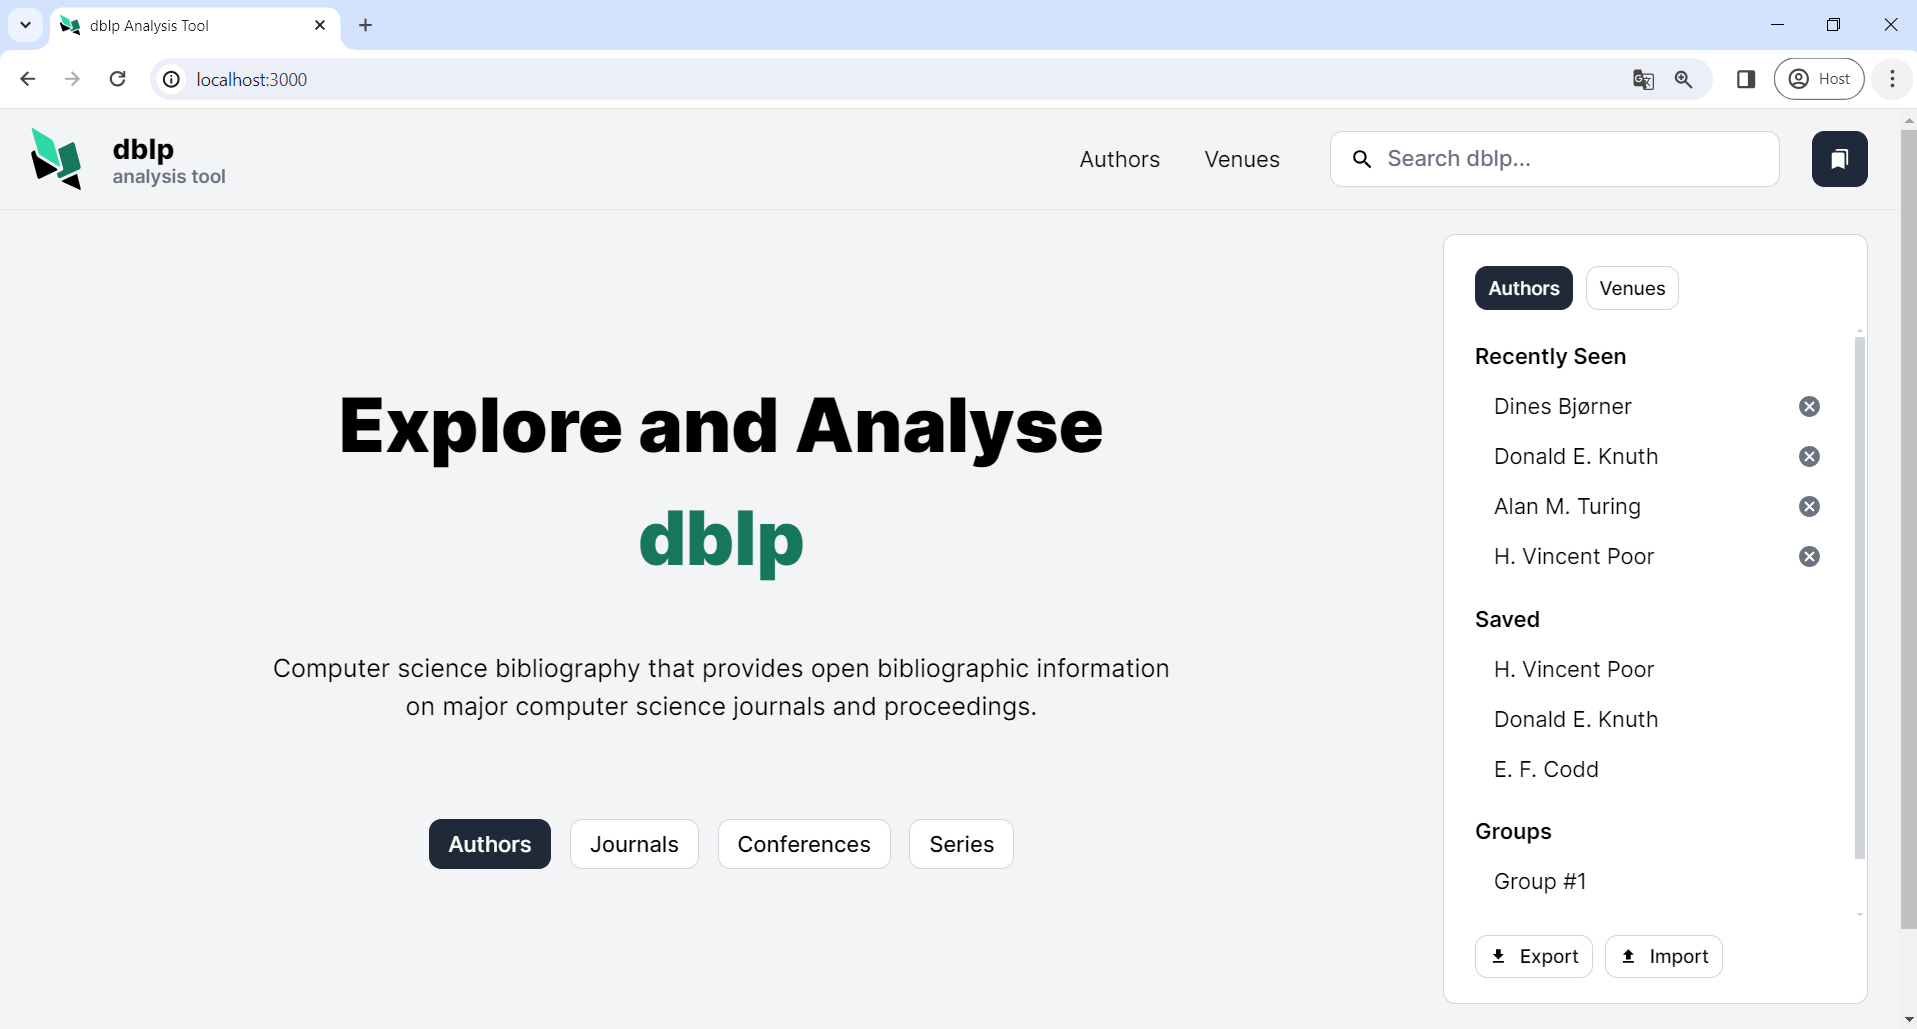
\includegraphics[width=\textwidth]{uvodni_stranka}
\caption{Úvodní stránka aplikace s~otevřeným postranním menu}\label{fig:uvodni_stranka}
\end{center}
\end{figure}

Uložené autory, skupiny autorů a~proudy publikací si můžeme nechat vyexportovat nebo opětovně naimportovat odpovídajícími tlačítky ve spodní části menu. Před vykonáním exportu si lze zvolit, jaké konkrétní položky se mají exportovat. Obdobně i~při importu. Položky se exportují do souboru ve formátu JSON.

\subsection{Vyhledávání}

Vyhledávač autorů a~proudů publikací v~této aplikaci funguje stejně jako ten v~DBLP. Porovnává tedy každý hledaný výraz jako předponu potenciálního výsledku vyhledávání. Jestliže hledaný výraz obsahuje více slov oddělených prázdným znakem nebo znakem~\uv{+}, pak všechny musí být předponami v~hledaném výsledku. Nerozlišují se velká a~malá písmena a~ani diakritika. Vyhledávání není fulltextové.

Vyhledávací dialog (viz obrázek~\ref{fig:vyhledavaci_dialog}) obsahuje především textové pole pro zadání hledaného výrazu s možností výběru, zda se mají vyhledávat autoři nebo proudy publikací. Po zadání výrazu se v~dialogu ještě zobrazuje seznam slov, na která lze výraz doplnit, a~seznam nejpravděpodobněji hledaných záznamů. Pokud takový záznam zvolíme, jsme ihned přesměrováni na odpovídající stránku autora, respektive proudu publikací. Jinak jsme při potvrzení hledaného výrazu přesměrováni na stránku se všemi výsledky hledání. Jestliže nezadáme žádný výraz, je vypsán odpovídající index. Stránka s~výsledky vyhledávání proudů publikací je rozdělena na tři sekce podle typů proudů -- časopisy, konference a~série.

\begin{figure}[H]
\begin{center}
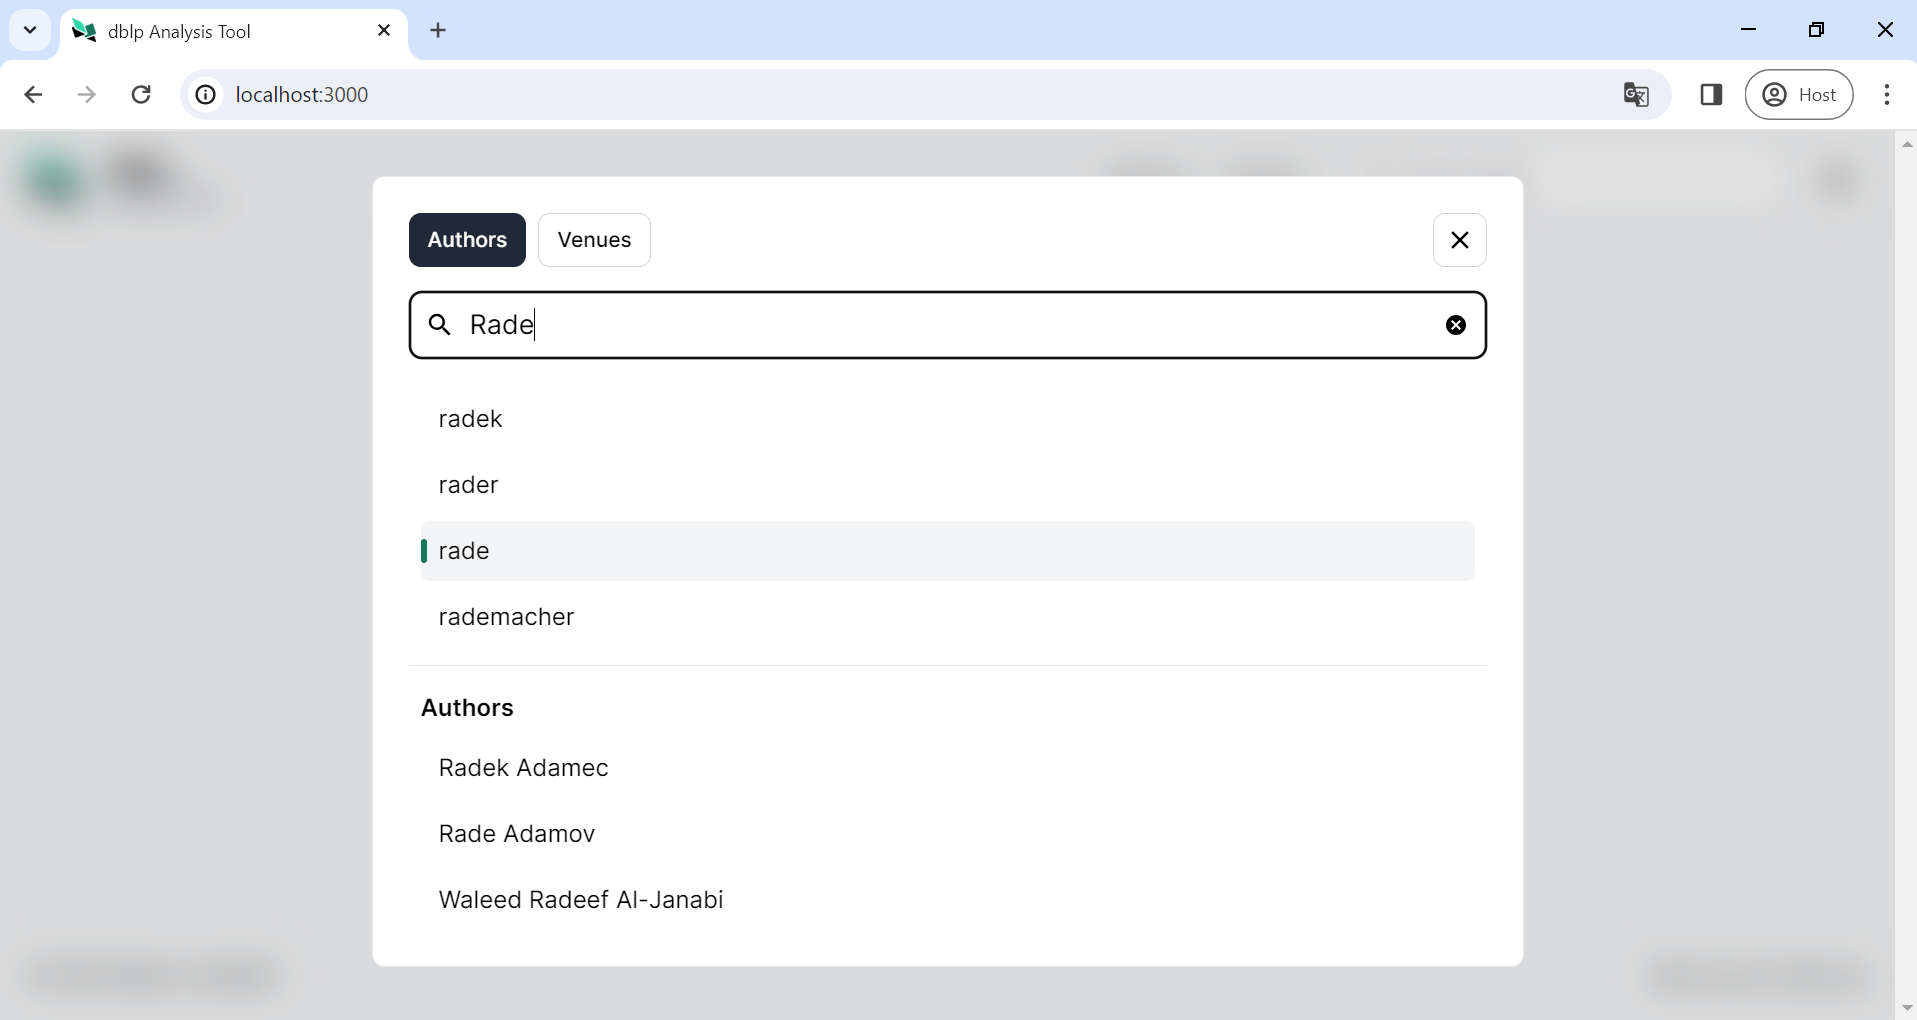
\includegraphics[width=\textwidth]{vyhledavaci_dialog}
\caption{Vyhledávací dialog v aplikaci}\label{fig:vyhledavaci_dialog}
\end{center}
\end{figure}

\subsection{Stránka autora}

Stránka autora je rozdělena do několika sekcí. První je hlavička, ve které nalezneme zejména autorovo jméno, případný alias, příslušnost k~univerzitě a~odkazy na různé domovské stránky autora. Vždy je zde minimálně odkaz na stránku autora v~DBLP. Dále jsou v~hlavičce ještě tři tlačítka pro: 
\begin{itemize}
\item uložení autora,
\item zobrazení dialogu pro přidání autora do skupiny,
\item export metadat autora do souboru ve formátu JSON.
\end{itemize}

Po hlavičce následuje sekce se seznamem autorů stejného jména a~sekce se seznamem ocenění. Ne u~všech autorů jsou tyto sekce k~dispozici. Příklad úvodní části stránky můžeme vidět na obrázku~\ref{fig:stranka_autora_hlavicka}. 

\begin{figure}[H]
\begin{center}
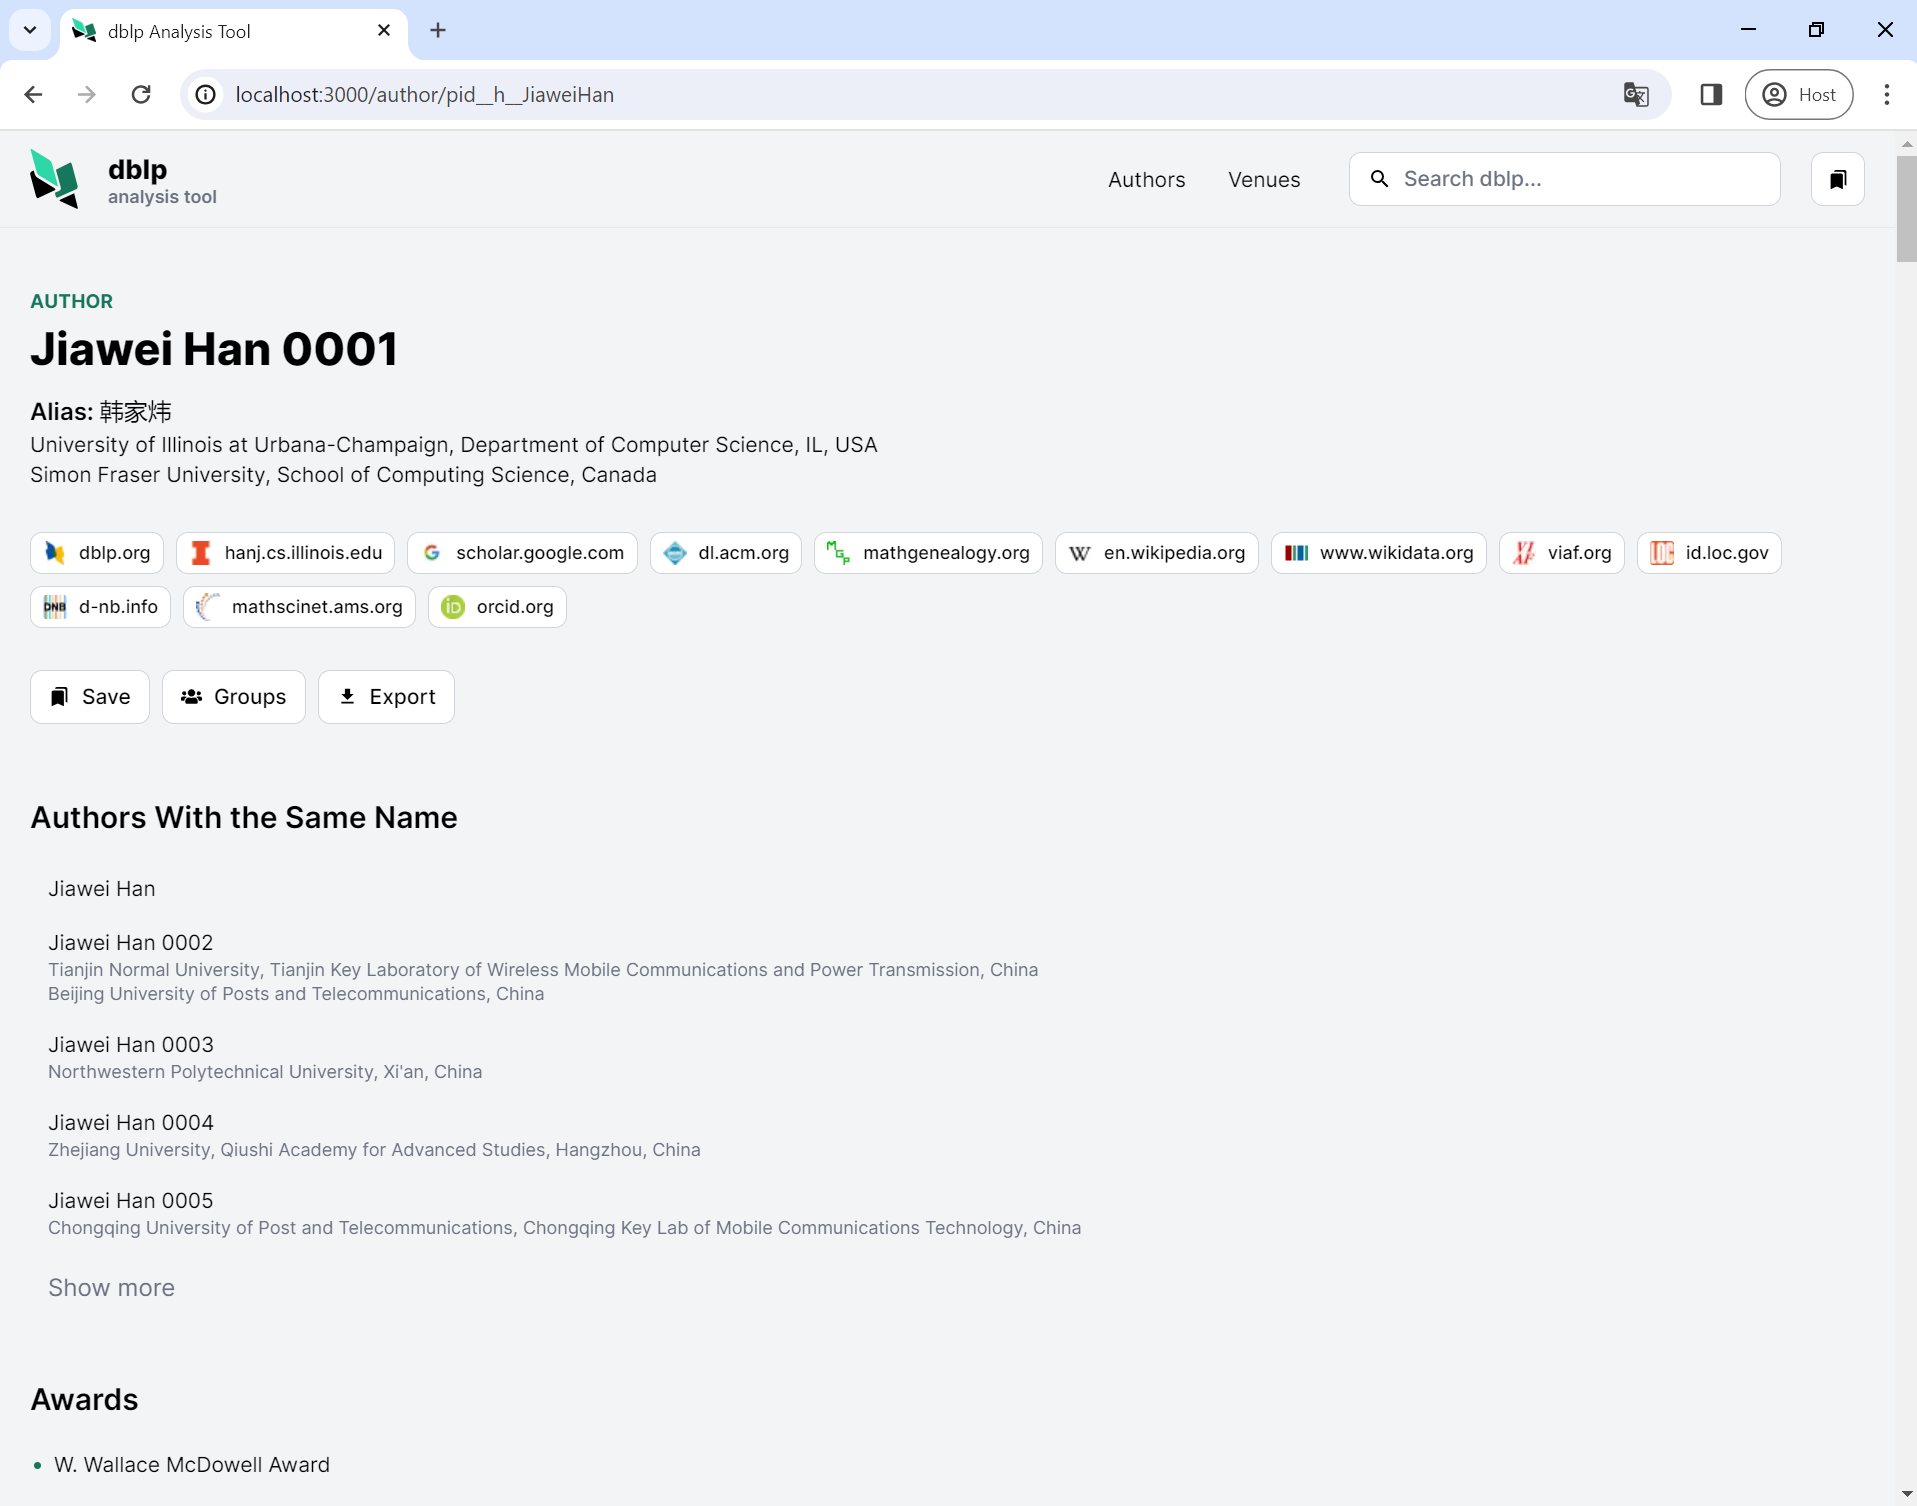
\includegraphics[width=\textwidth]{stranka_autora_hlavicka}
\caption{Stránka autora Jiawei Han 0001 v~aplikaci}\label{fig:stranka_autora_hlavicka}
\end{center}
\end{figure}

Další sekcí je sekce s~různými statistikami publikací. Titulek sekce je zároveň odkazem na stránku se všemi publikacemi autora. V~této sekci nalezneme vypsány nejvýše tři nejnovější publikace autora a~tři různé statistiky publikací:
\begin{itemize}
\item počty publikací jednotlivých typů (viz obrázek~\ref{fig:stranka_autora_kolac}),
\item počty publikací publikovaných v~jednotlivých letech,
\item přehled proudů publikací, do kterých jsou publikace zařazeny.
\end{itemize}

Všechny statistiky jsou prezentovány tabulkou a~alespoň jedním typem grafu. Pokud ve sloupcovém grafu klikneme na některý sloupec, jsme přesměrováni na stránku s~vyfiltrovanými publikacemi, které danému sloupci odpovídají. Obdobně funguje i~koláčový graf.

\begin{figure}[H]
\begin{center}
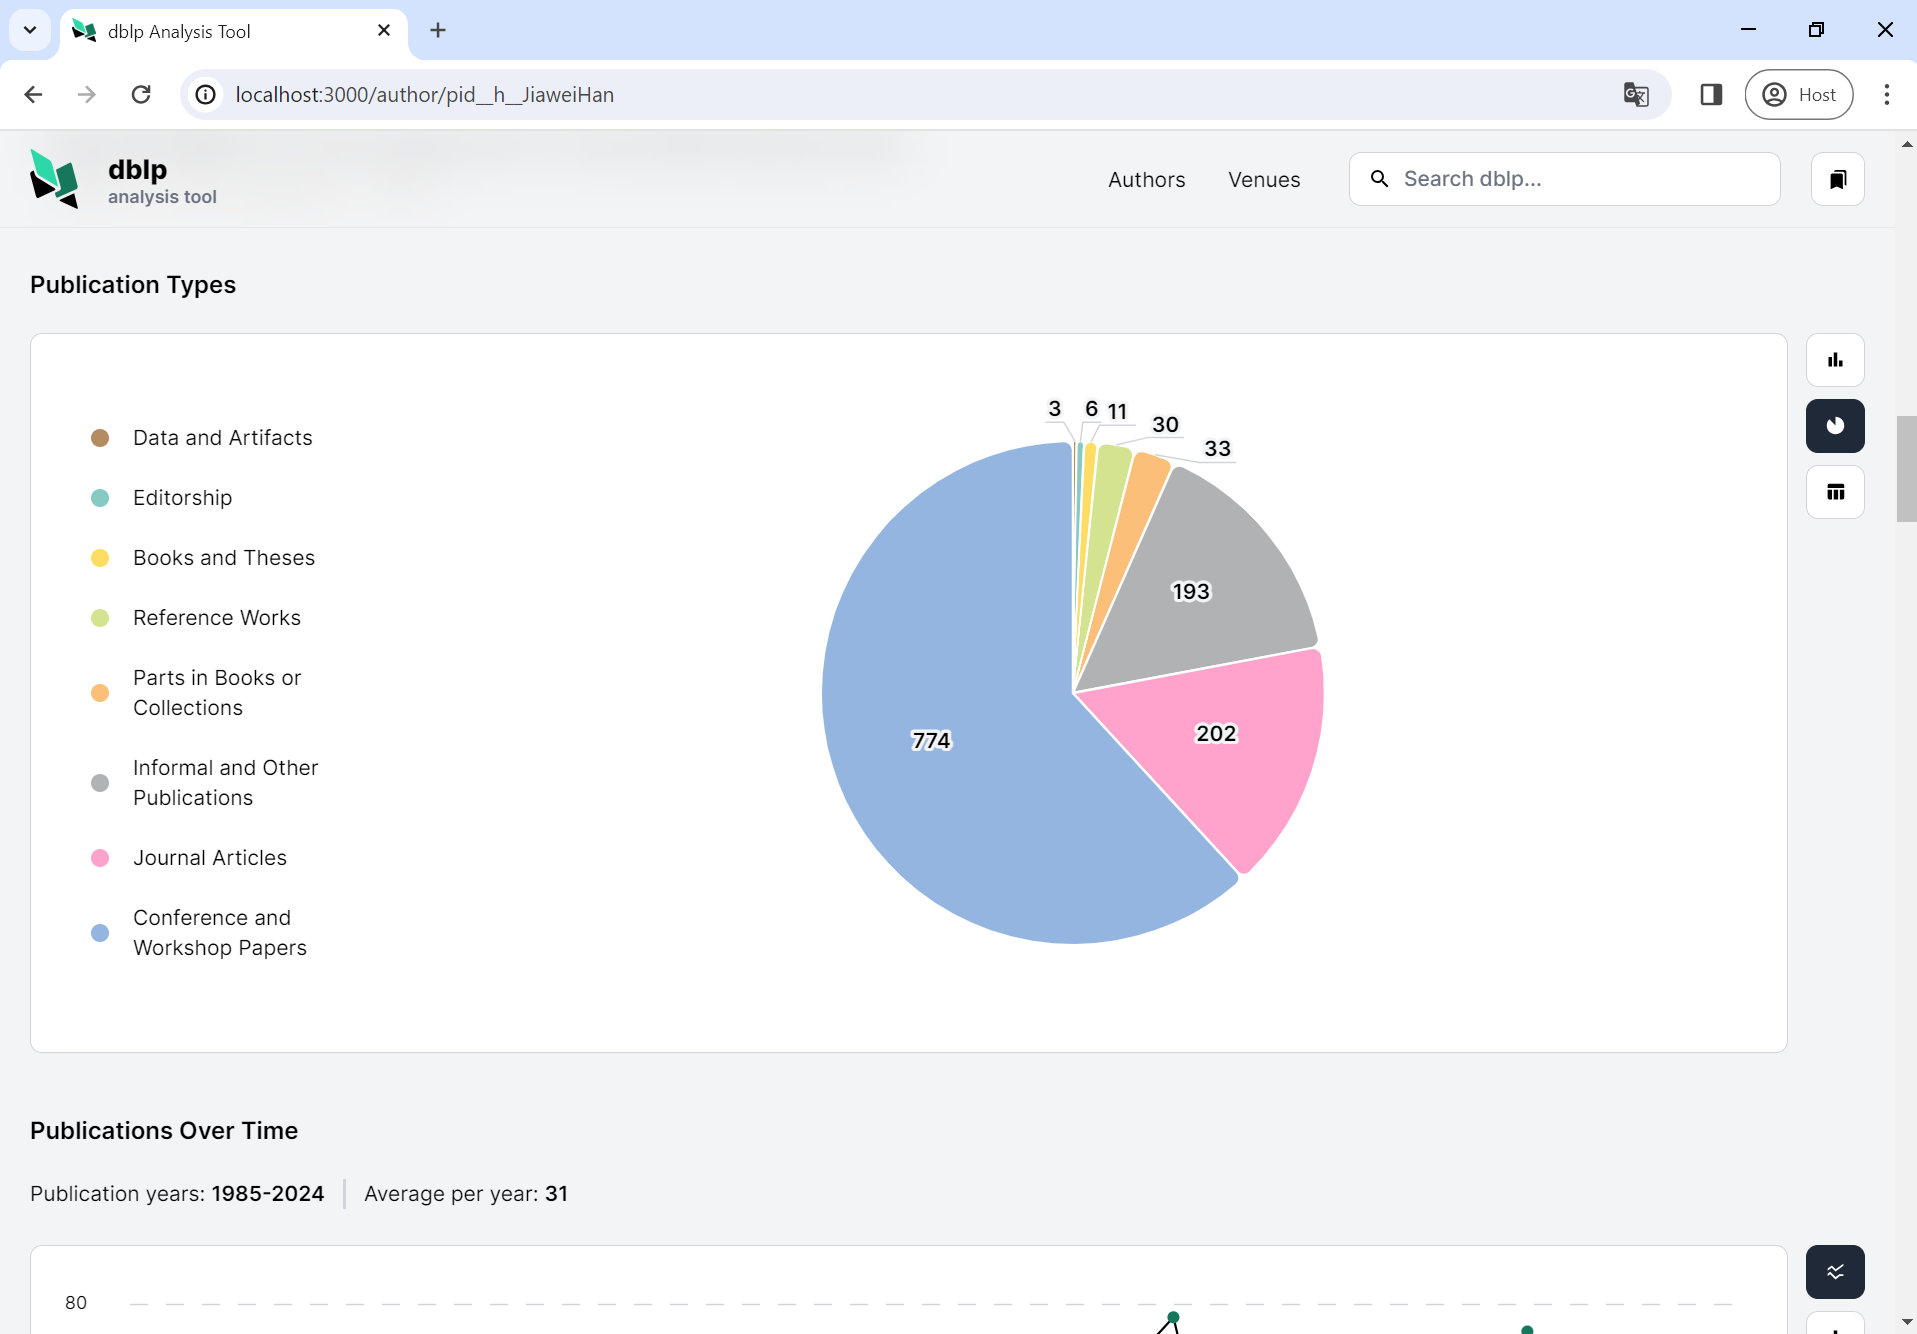
\includegraphics[width=\textwidth]{stranka_autora_kolac}
\caption{Komponenta koláčového grafu, který vizualizuje počty publikací autora jednotlivých typů.}\label{fig:stranka_autora_kolac}
\end{center}
\end{figure}

Poslední sekcí je sekce s~grafem spoluautorství a~tabulkou všech spoluautorů. Graf spoluautorství je popsán v~kapitole~\ref{sec:graf_spoluautorstvi}. V~tabulce spoluautorů je u~každého autora uveden počet společných publikací se zobrazeným autorem a~počet společných spoluautorů těchto publikací. Nemusí se však nutně jednat o~celkový počet společných spoluautorů. Dva různí autoři totiž mohou mít společného spoluautora a~přitom všichni tři nemusí být autory stejné publikace.

\subsection{Stránka skupiny autorů}

Stránka skupiny autorů je stejně jako stránka autora rozdělena do několika sekcí. V~hlavičce nalezneme název skupiny a~tlačítka pro: 
\begin{itemize}
\item přejmenování skupiny,
\item smazání skupiny,
\item export metadat členů skupiny do souboru ve formátu JSON.
\end{itemize}

Za hlavičkou následuje přehled všech členů skupiny, ze kterého si můžeme vybrat konkrétní členy, jejichž metadata mají být prezentována. Rychlost načtení metadat členů závisí na tom, zda jsou zrovna uložena v~mezipaměti. Pokud nejsou, tak je rychlost významně omezena uměle zavedeným čekáním mezi poslanými požadavky na DBLP.

Další sekcí je sekce se statistikami publikací vybraných členů skupiny. Titulek sekce je zároveň odkazem na stránku se všemi publikacemi skupiny. Sekce obsahuje stejné statistiky jako na stránce autora a~navíc ještě statistiku počtů publikací jednotlivých členů. Publikace je možné v~této statistice filtrovat. Poslední sekce obsahuje graf spoluautorství (viz~kapitola~\ref{sec:graf_spoluautorstvi}) a~tabulku všech spoluautorů vybraných členů. V~tabulce spoluautorů je u~každého autora uveden celkový počet publikací, které jsou společné s~alespoň jedním z~vybraných členů skupiny, a~počet společných spoluautorů těchto publikací.

\subsection{Stránka proudu publikací}

V~hlavičce stránky proudu publikací nalezneme název proudu, odkaz na stránku proudu v~DBLP a~tlačítka pro:
\begin{itemize}
\item uložení proudu publikací,
\item export metadat proudu publikací a~případných svazků do souboru ve formátu JSON.
\end{itemize}

Po hlavičce následuje sekce se statistikou počtu publikací publikovaných v~jednotlivých letech v~daném proudu publikací a~statistikou nejaktivnějších autorů v~daném proudu publikací. Další obsah stránky závisí na typu proudu publikací:
\begin{itemize}
\item Dělící se na svazky -- Je vypsán přehled všech svazků s~možností jejich výběru. Příklad takového přehledu můžeme vidět na~obrázku~\ref{fig:stranka_proudu_publikaci_svazky}. Za přehledem následuje sekce se statistikami publikací vybraných svazků a~sekce s~grafem spoluautorství a~tabulkou všech autorů vybraných svazků.
\item Obsahující publikace představující svazky -- Je možné si vybrat mezi zobrazením metadat publikací představujících svazky a~zobrazením metadat publikací vybraných svazků. V~obou případech je zobrazena sekce se statistikami publikací a~sekce s~grafem spoluautorství a~tabulkou všech autorů.
\item Nedělící se na svazky -- Je zobrazena sekce se statistikami publikací a~sekce s~grafem spoluautorství a~tabulkou všech autorů.
\end{itemize}

Graf spoluautorství je popsán v~kapitole~\ref{sec:graf_spoluautorstvi}. V~tabulkách autorů je u~každého autora uveden celkový počet jeho publikací z daného proudu publikací nebo svazku a~počet společných spoluautorů těchto publikací. Metadata každého svazku si můžeme zobrazit odděleně na samostatné stránce. Taková stránka opět obsahuje sekci se statistikami publikací daného svazku a~sekci s~grafem spoluautorství (viz~kapitola~\ref{sec:graf_spoluautorstvi}) a~tabulkou všech autorů daného svazku.

\begin{figure}[H]
\begin{center}
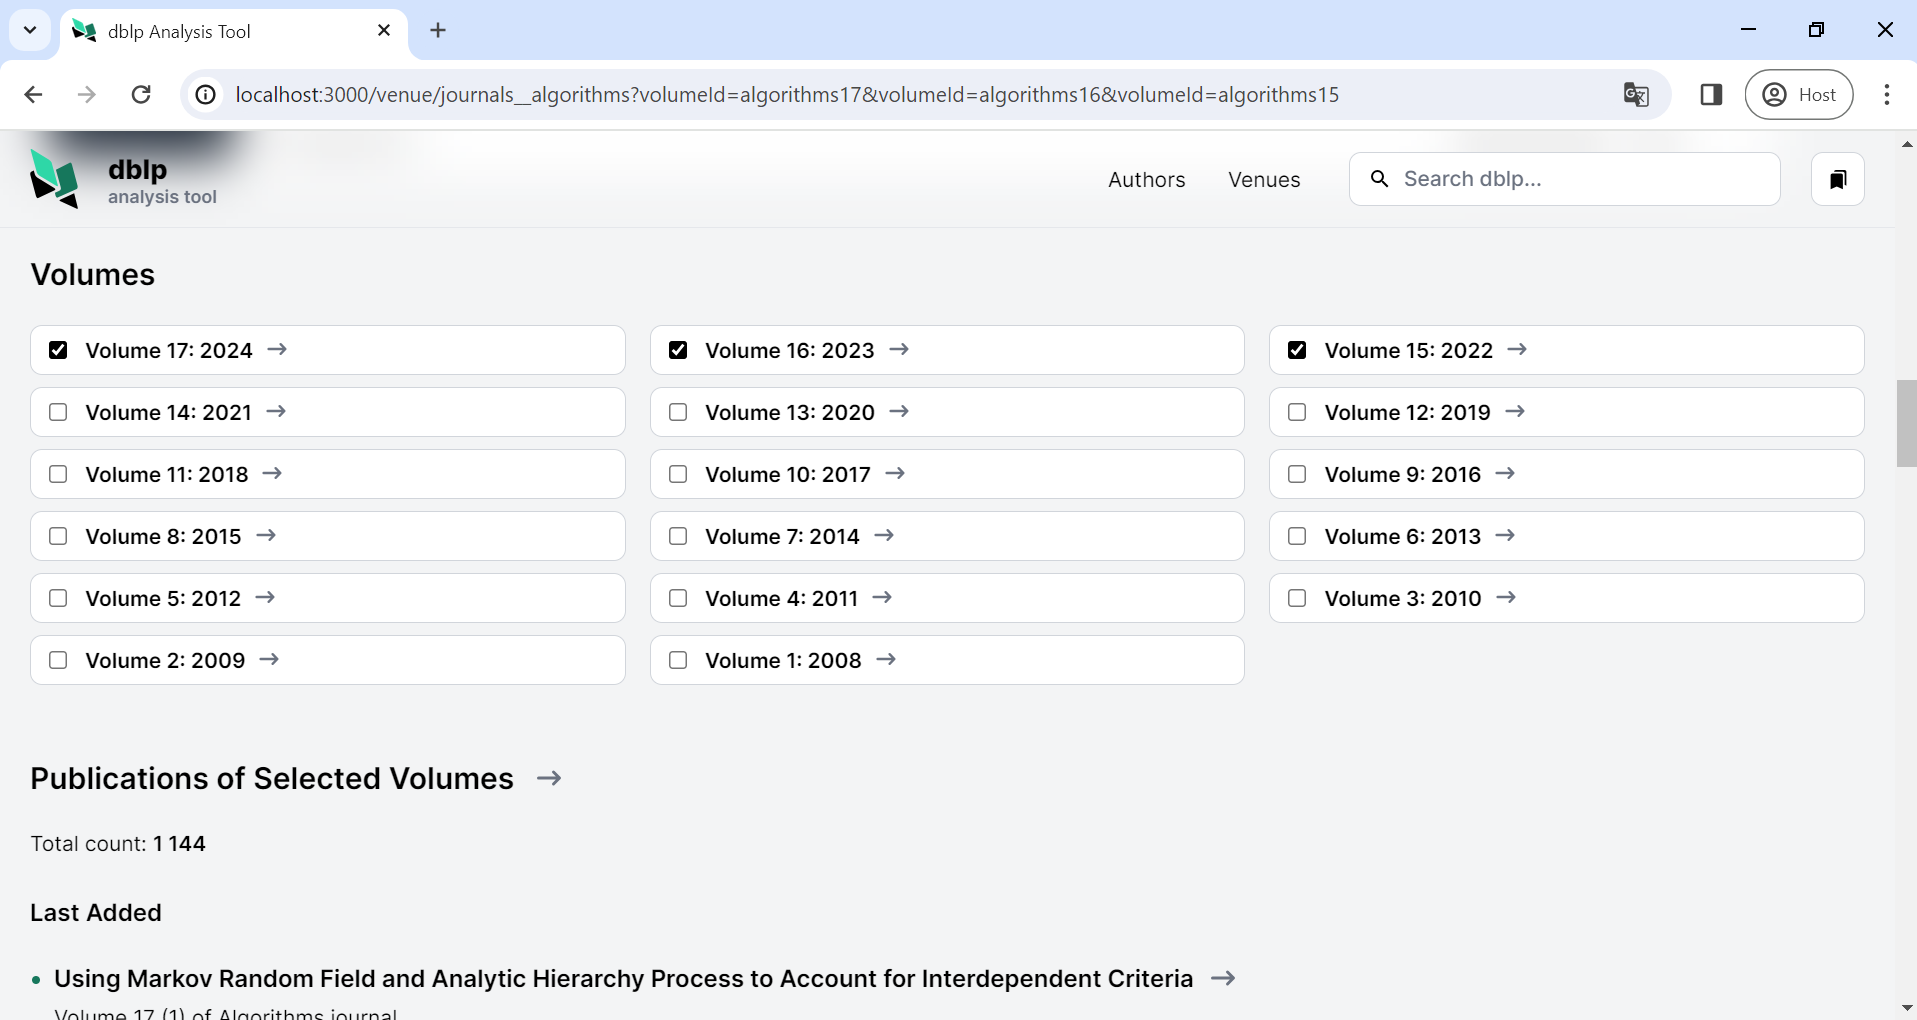
\includegraphics[width=\textwidth]{stranka_proudu_publikaci_svazky}
\caption{Přehled všech svazků proudu publikací s~možností jejich výběru}\label{fig:stranka_proudu_publikaci_svazky}
\end{center}
\end{figure}

\subsection{Stránky publikací a~filtrování}

Pro přehled všech publikací autora, skupiny autorů nebo proudu publikací nabízí aplikace samostatné stránky. Na těchto stránkách najdeme kromě výpisu všech publikací i~stejné statistiky publikací jako na odpovídajících stránkách autora, skupiny autorů nebo proudu publikací. Zobrazené publikace můžeme v~aplikaci filtrovat podle čtyř různých typů filtrů:
\begin{itemize}
\item typ publikace,
\item rok vydání publikace,
\item proud publikací, do kterého je publikace zařazena,
\item autor publikace.
\end{itemize}

Pokud vybereme více filtrů stejného typu, pak musí vybraná publikace splňovat alespoň jeden z těchto filtrů. U autorů si však můžeme vynutit, že má publikace splňovat všechny filtry (tedy obsahovat všechny zvolené autory). Pokud vybereme dva filtry různých typů, pak musí vybraná publikace splňovat oba filtry zároveň. Jestliže tedy vybereme například filtry pro rok \uv{2000} a~\uv{2001} a~pro typ publikace \uv{Journal Articles}, jsou zobrazeny pouze články vydané v~roce 2000 nebo 2001. Dialog pro výběr filtrů můžeme vidět na obrázku~\ref{fig:filtrovaci_dialog}.

\begin{figure}[H]
\begin{center}
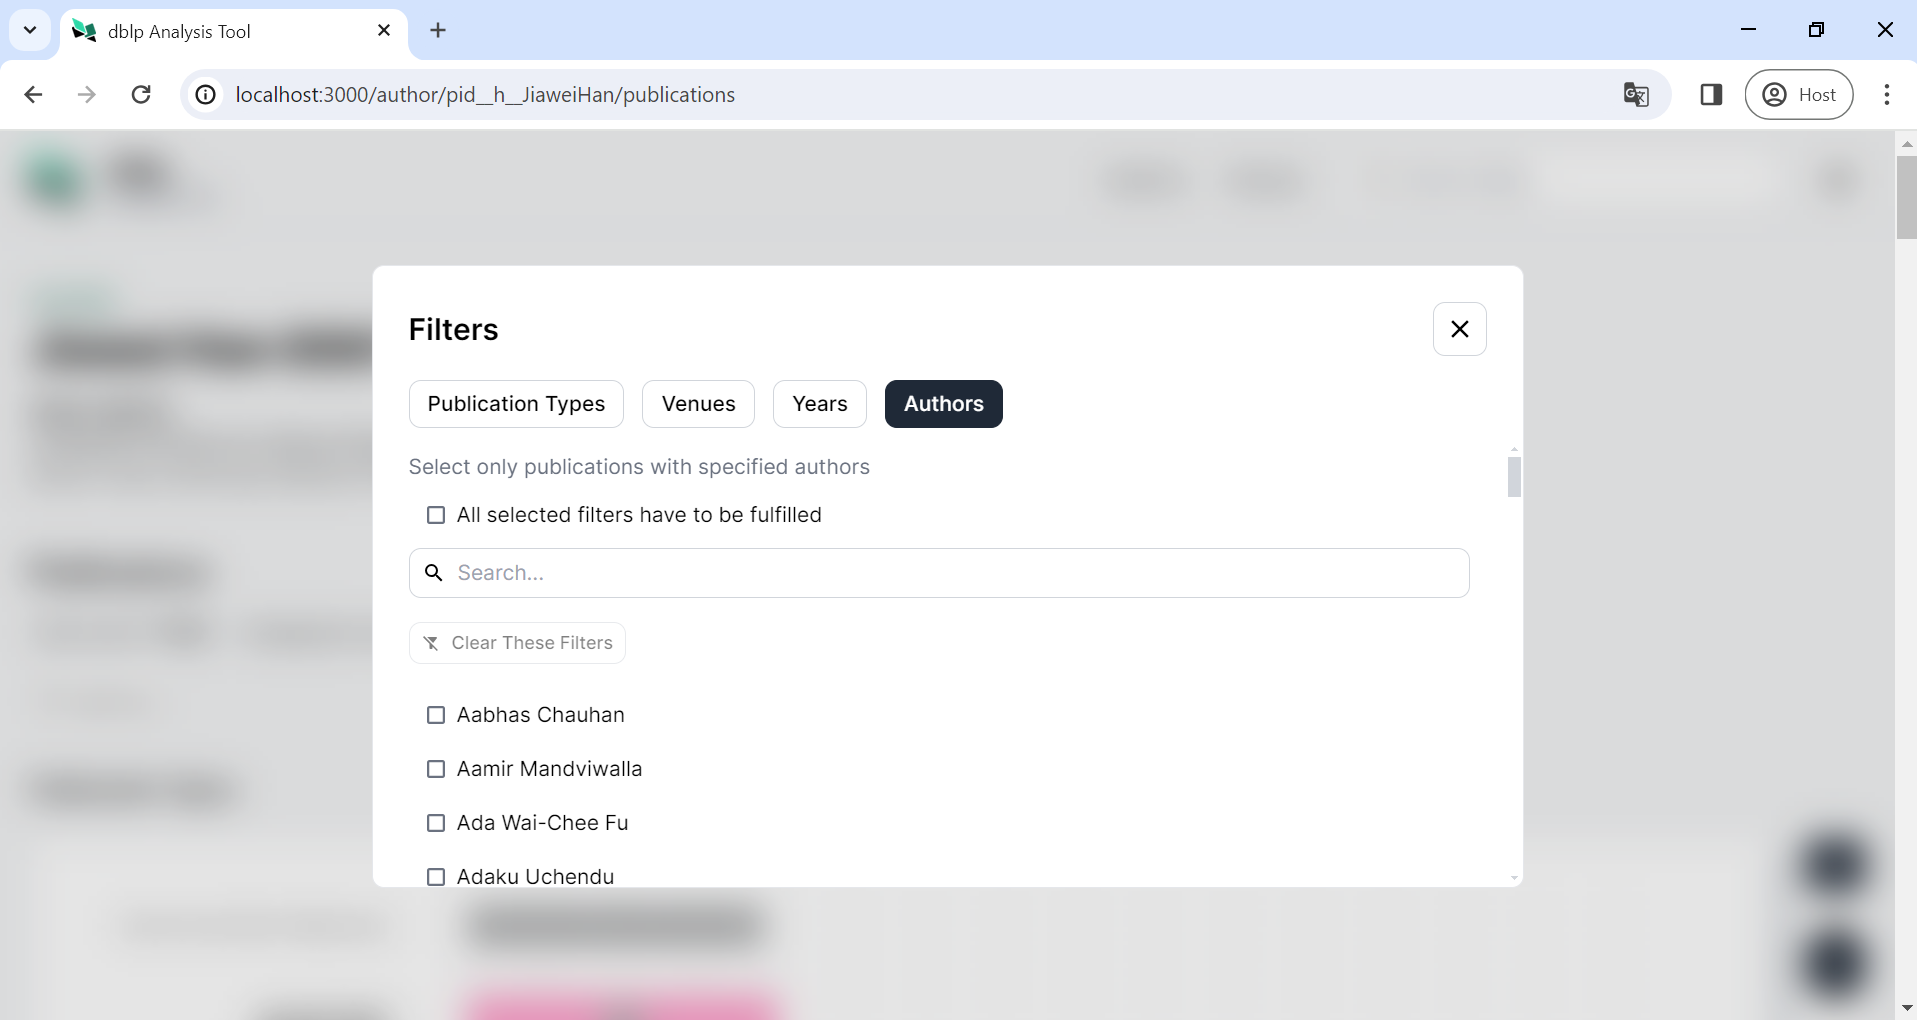
\includegraphics[width=\textwidth]{filtrovaci_dialog}
\caption{Dialog pro výběr filtrů publikací}\label{fig:filtrovaci_dialog}
\end{center}
\end{figure}

\subsection{Graf spoluautorství} \label{sec:graf_spoluautorstvi}

Graf spoluautorství je vždy tvořen všemi autory publikací z~nějaké \textit{množiny publikací}. V~případě stránky autora nebo skupiny autorů se jedná o~množinu publikací všech originálních autorů. \textit{Originální autor} je autor, jehož všechny publikace jsou zahrnuty do množiny publikací. Aktuálně zobrazený autor na stránce autora a~všichni vybraní členové skupiny autorů na stránce skupiny autorů jsou vždy považováni za originální autory. Další originální autory lze zařadit manuálně. V~případě stránky proudu publikací je množina tvořena buď publikacemi daného proudu, nebo publikacemi vybraných svazků.

Uzly grafu představují autory publikací z~dané množiny publikací. Neorientované hrany grafu představují relaci spoluautorství. Mezi dvěma autory existuje hrana pouze v~případě, že jsou spoluautory stejné publikace z~dané množiny publikací. Může tak nastat situace, kdy jsou dva autoři spoluautory stejné publikace, ale v~grafu mezi nimi není hrana, protože tato publikace není zahrnuta v~dané množině publikací. Ohodnocení hran představuje počet společných publikací dvou autorů z~dané množiny publikací.

Ukázku komponenty grafu můžeme vidět na obrázku~\ref{fig:graf_spoluautorstvi}. Jestliže graf obsahuje dva a~více originálních autorů, můžeme si nechat zobrazit pouze jejich společné spoluautory. Autory lze v~grafu taktéž vyhledávat a~filtrovat. Filtrování funguje obdobně jako v~případě publikací. Můžeme si díky němu zobrazit pouze:
\begin{itemize}
\item vybrané autory,
\item autory určitého typu publikace,
\item autory publikace vydané v~určitém roce,
\item autory publikace zařazené do určitého proudu publikací.
\end{itemize}

\begin{figure}[H]
\begin{center}
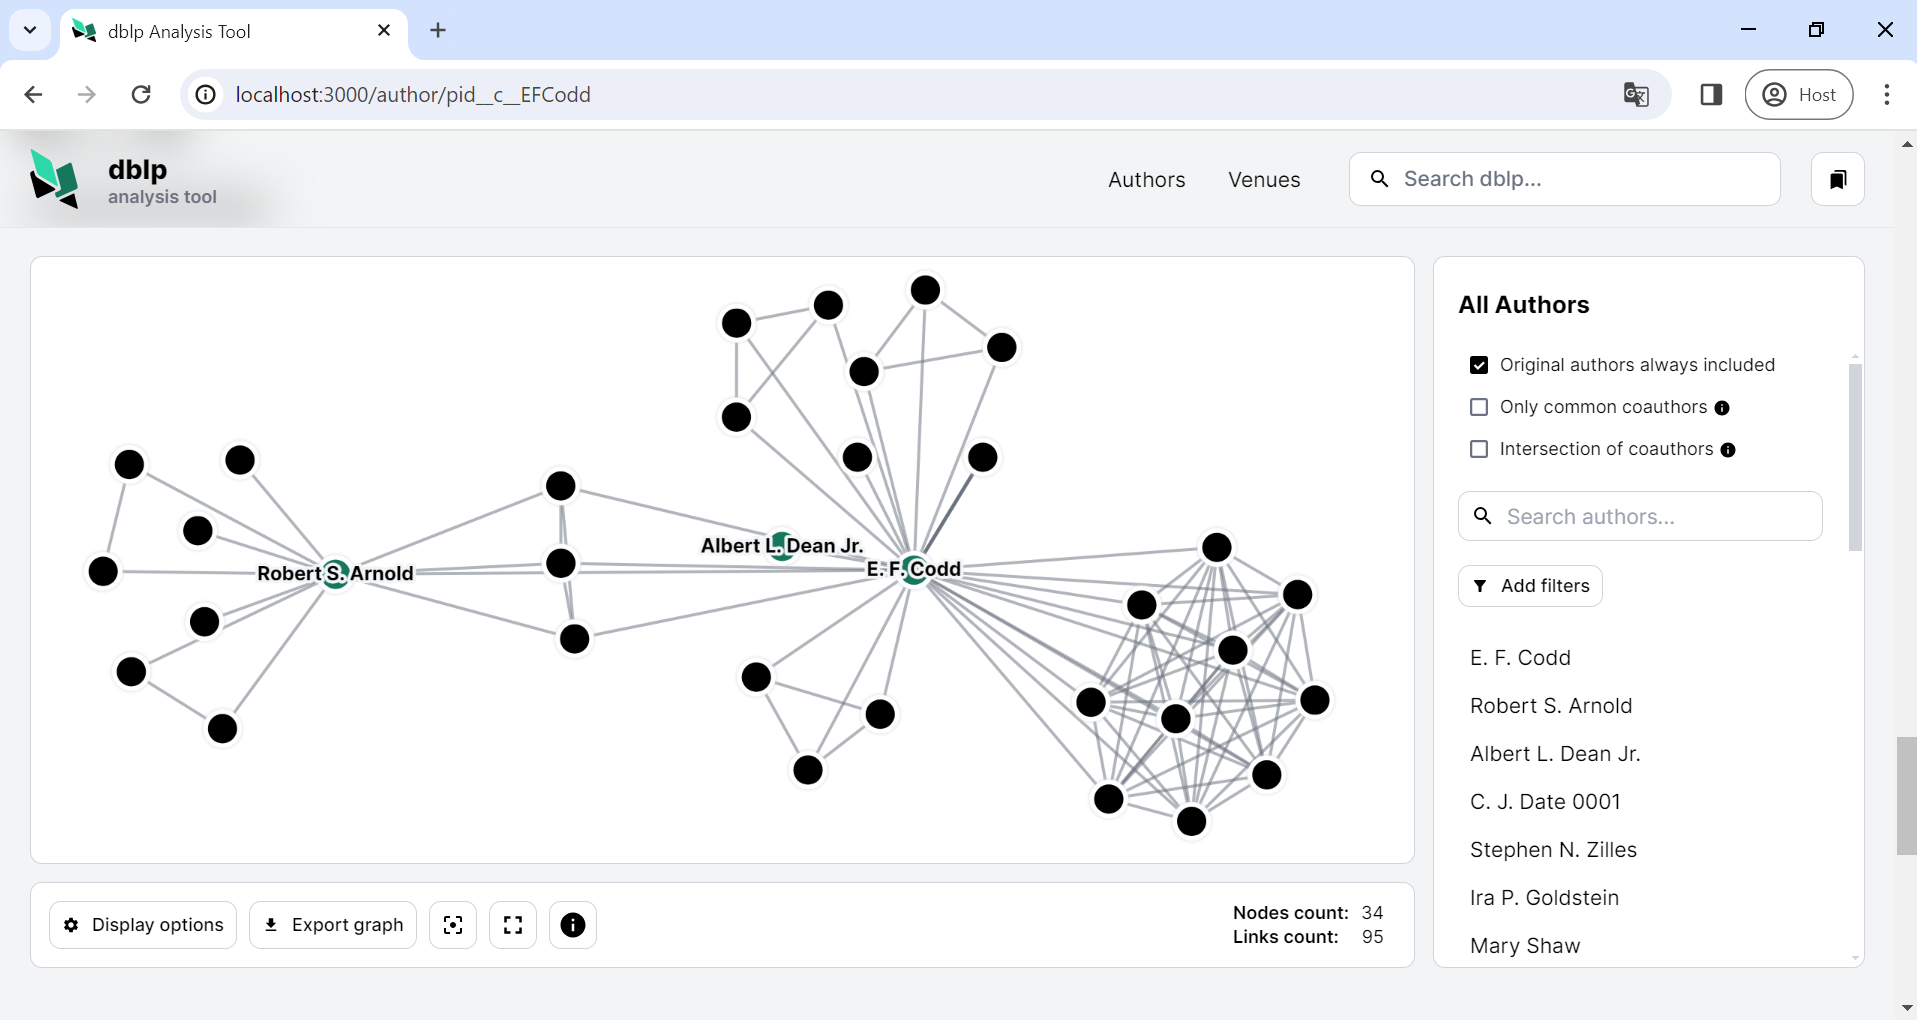
\includegraphics[width=\textwidth]{graf_spoluautorstvi}
\caption{Komponenta grafu spoluautorství}\label{fig:graf_spoluautorstvi}
\end{center}
\end{figure}

Komponentě grafu můžeme nastavit různé možnosti zobrazení, jako například možnosti zobrazení odfiltrovaných autorů, popisků uzlů nebo ohodnocení hran. Pro pohodlnější práci s~grafem si navíc můžeme jeho komponentu nechat roztáhnout na celou obrazovku. Graf je možné exportovat do řady různých formátů:
\begin{itemize}
\item JSON,
\item CSV -- buď jako seznam hran, nebo jako matici (u~grafů s~nejvýše 4000 uzly),
\item GraphViz DOT,
\item GDF,
\item GML,
\item GraphML,
\item GEXF.
\end{itemize}

Na každého autora v~grafu je možné kliknout a nechat si tak zobrazit přehled všech jeho spoluautorů. Tito spoluautoři jsou rozdělení do dvou skupin -- spoluautoři, kteří jsou společní s~nějakým originálním autorem, a~spoluautoři, kteří nejsou. U~spoluautorů jsou zobrazena ohodnocení případných hran, tedy počty společných publikací z~dané množiny publikací. Ohodnocení hrany se zobrazí, i~pokud na ni v~grafu najedeme myší.

%% Závěry práce. V jazyce práce a anglicky. Text pro jiný než
%% nastavený jazyk práce (nepovinným parametrem language makra
%% \documentclass, výchozí český) se zadává použitím makra s uvedením
%% jazyka jako nepovinného parametru.
\begin{kiconclusions}

%% jaký je výsledek

Výsledkem této bakalářské práce je webová aplikace, která umožňuje provádět analýzu nad daty z~DBLP databáze. Aplikace plní svůj účel. Nabízí řadu vizualizací různých statistik a~vztahů mezi daty. Zvlášť hodnotná může být pro uživatele komponenta grafu spoluautorství umožňující snazší pochopení vztahů mezi jednotlivými autory. Uživatelské rozhraní aplikace je přehledné a~přívětivé, čímž taktéž napomáhá k~snadnějšímu pochopení analyzovaných dat. Všechna analyzovaná data má uživatel možnost si stáhnout. Nejen architekturu aplikace, ale i~její uživatelské rozhraní jsem navrhl tak, aby případné rozšíření aplikace o~nové funkcionality bylo co nejjednodušší.

\end{kiconclusions}

\begin{kiconclusions}[english]
The result of this bachelor’s thesis is a web application that allows for analysis of data from the DBLP database. The application fulfills its purpose. It offers a range of visualizations of various statistics and relationships between data. Particularly valuable for users may be the co-authorship graph component that enables easier understanding of the relationships between individual authors. The user interface of the application is clear and user-friendly, which also helps to more easily understand the analyzed data. Users have the option to download the analyzed data. I~designed not only the application’s architecture but also its user interface to make any potential expansion of the application with new functionalities as simple as possible.
\end{kiconclusions}

%% Přílohy obsahu textu práce, za makrem \appendix.
\appendix

\section{Zprovozněná aplikace}

Pro účely testování je vytvořená aplikace v době odevzdání této práce zprovozněna na adrese \href{http://158.194.92.113/}{http://158.194.92.113/}, případně je možné ji zprovoznit z přiložených zdrojových kódů.

%% Obsah elektronických dat. Poslední příloha.
\section{Obsah elektronických dat} \label{sec:ObsahData}

\begin{description}

\item[\texttt{text/}] \hfill \\
  Adresář obsahující text bakalářské práce ve formátu PDF a~zdrojové kódy tohoto textu.

\item[\texttt{src/}] \hfill \\
  Adresář obsahující zdrojové kódy aplikace.

\item[\texttt{README.txt}] \hfill \\
  Textový soubor obsahující postup zprovoznění aplikace.

\end{description}


%% -------------------------------------------------------------------

%% Sazba volitelného seznamu zkratek, za přílohami.
%% \printglossary

%% Sazba povinné bibliografie, za přílohami (případně i za seznamem
%% zkratek). Při použití BibLaTeXu použijte makro
%% \printbibliography. jinak prostředí thebibliography. Ne obojí!

%% Sazba i v textu necitovaných zdrojů, při použití
%% BibLaTeXu. Volitelné.
\nocite{*}
%% Vlastní sazba bibliografie při použití BibLaTeXu.
\printbibliography

%% Sazba volitelného rejstříku, za bibliografií.
\printindex

\end{document}

%%% Local Variables:
%%% mode: latex
%%% TeX-master: t
%%% End:
